% Settings for the default beamer theme
\documentclass[english, aspectratio=169]{beamer}
\usepackage[T1]{fontenc}
\usepackage[utf8]{inputenc}
\usepackage{tabularx}
\usepackage{babel}
\usepackage[ruled,vlined]{algorithm2e}
\SetAlgorithmName{Algoritmus}{algoritmus}{List of Algorithms}
\setcounter{secnumdepth}{3}
\setcounter{tocdepth}{3}

\makeatletter

\newcommand\makebeamertitle{\frame{\maketitle}}

% (ERT) argument for the TOC
\AtBeginDocument{%
  \let\origtableofcontents=\tableofcontents
  \def\tableofcontents{\@ifnextchar[{\origtableofcontents}{\gobbletableofcontents}}
  \def\gobbletableofcontents#1{\origtableofcontents}
}

% Theme settings
\usetheme{Frankfurt}
\usecolortheme{default}
\usefonttheme[onlymath]{serif}

% Template settings
\setbeamertemplate{navigation symbols}{}
\setbeamertemplate{blocks}[rounded][shadow=false]
\setbeamertemplate{title page}[default][colsep=-4bp, rounded=true, shadow=false]
\makeatother

\begin{document}

% Title page
\section{Bevezetés}
\title[]{Üzleti Intelligencia}
\subtitle{5. Előadás: $Q$-tanulás}
\author[Kuknyó Dániel]{Kuknyó Dániel\\Budapesti Gazdasági Egyetem}
\date{2023/24\\1.félév}
\makebeamertitle

% Table of contents slide
\begin{frame}
\tableofcontents{}
\end{frame}

% Table of contents of the current section
\begin{frame}
\tableofcontents[currentsection]
\end{frame}

\begin{frame}{Bevezetés a $Q$-tanulásba}
A megerősítéses tanulásban a $Q_\pi(s,a)$ minőségfüggvény megadja, hogy mennyire jövedelmező az ügynöknek, ha $s$ állapotban állva, $a$ cselekvést végrehajtva majd onnan $\pi$ politikát követve mekkora a várható hozam.\par\smallskip
Ha adott minden állapotra és cselekvésre az optimális $Q(s,a)$ érték, onnan levezethető a $\pi_*$ optimális politika, amelynek várható hozama maximális.
\begin{center}
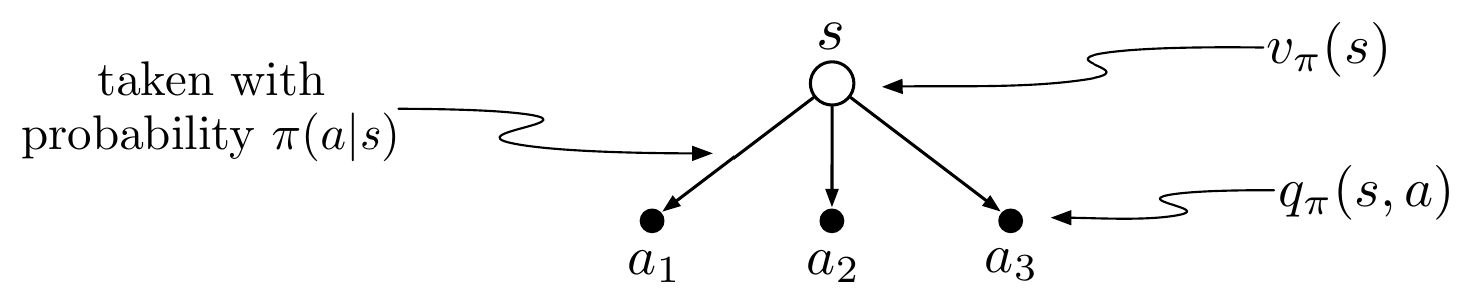
\includegraphics[width=12cm, keepaspectratio]{images/ql_1.png}
\begin{block}{}
\[
Q_\pi(s,a)=E_\pi \left[ G_t \vert s_t=s, a_t=a \right] = E_\pi \left[ \sum_{k=0}^\infty \gamma^kr_{t+k+1} \vert s_t=s, a_t=a \right]
\]
\end{block}
\end{center}
\end{frame}

\begin{frame}{$Q$-tanulás: politikafüggetlen TD irányítás}
\begin{columns}
\begin{column}{.75\textwidth}
A megerősítéses tanulásban az egyik nagy áttörést egy politikafüggetlen TD algoritmus kifejlesztése hozta el.\par\smallskip
Ebben az esetben a becsült állapot-cselekvés minőség függvény, $Q$, direkten becsüli meg  $q_*$ optimális állapot-cselekvés minőség függvényt a követett politikától teljesen függetlenül.
\begin{block}{$Q$-tanulás}
\[
Q(s,a) \leftarrow Q(s,a) + \alpha \left[ r + \gamma \underset{a'}{max}Q(s',a') - Q(s,a) \right]
\]
\end{block}
Az egyetlen különbség a SARSA algoritmusától, hogy a referencia a következő állapotból elérhető legjobb minőségű cselekvés értéke: $\underset{a}{max}Q(s_{t+1},a)$.
\end{column}
\begin{column}{.25\textwidth}
\begin{center}
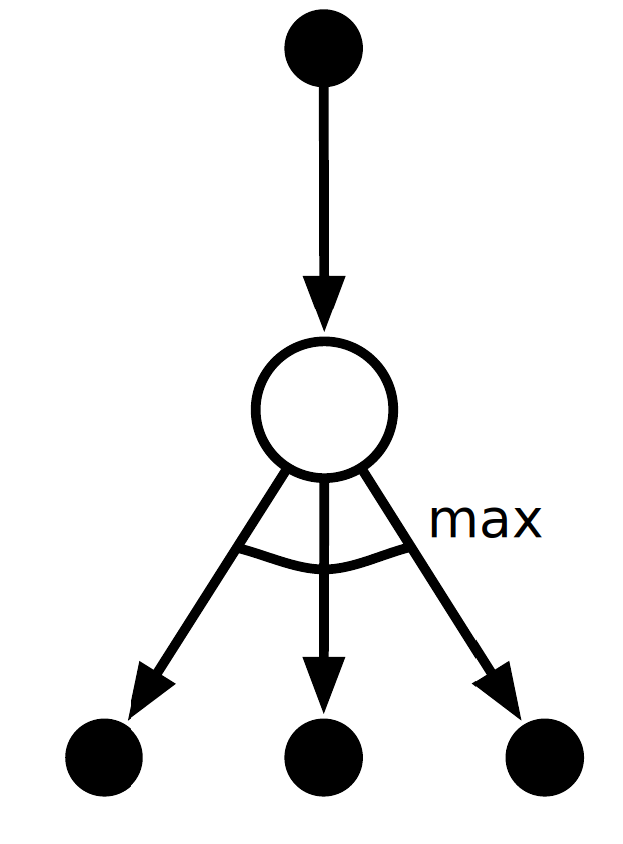
\includegraphics[width=3cm, keepaspectratio]{images/ql_2.png}
\end{center}
\end{column}
\end{columns}
\end{frame}

\begin{frame}{$Q$-tanulás eljárása}
\begin{columns}
\begin{column}{.5\textwidth}
\begin{center}
A $Q$-tanulás folyamata\par\medskip
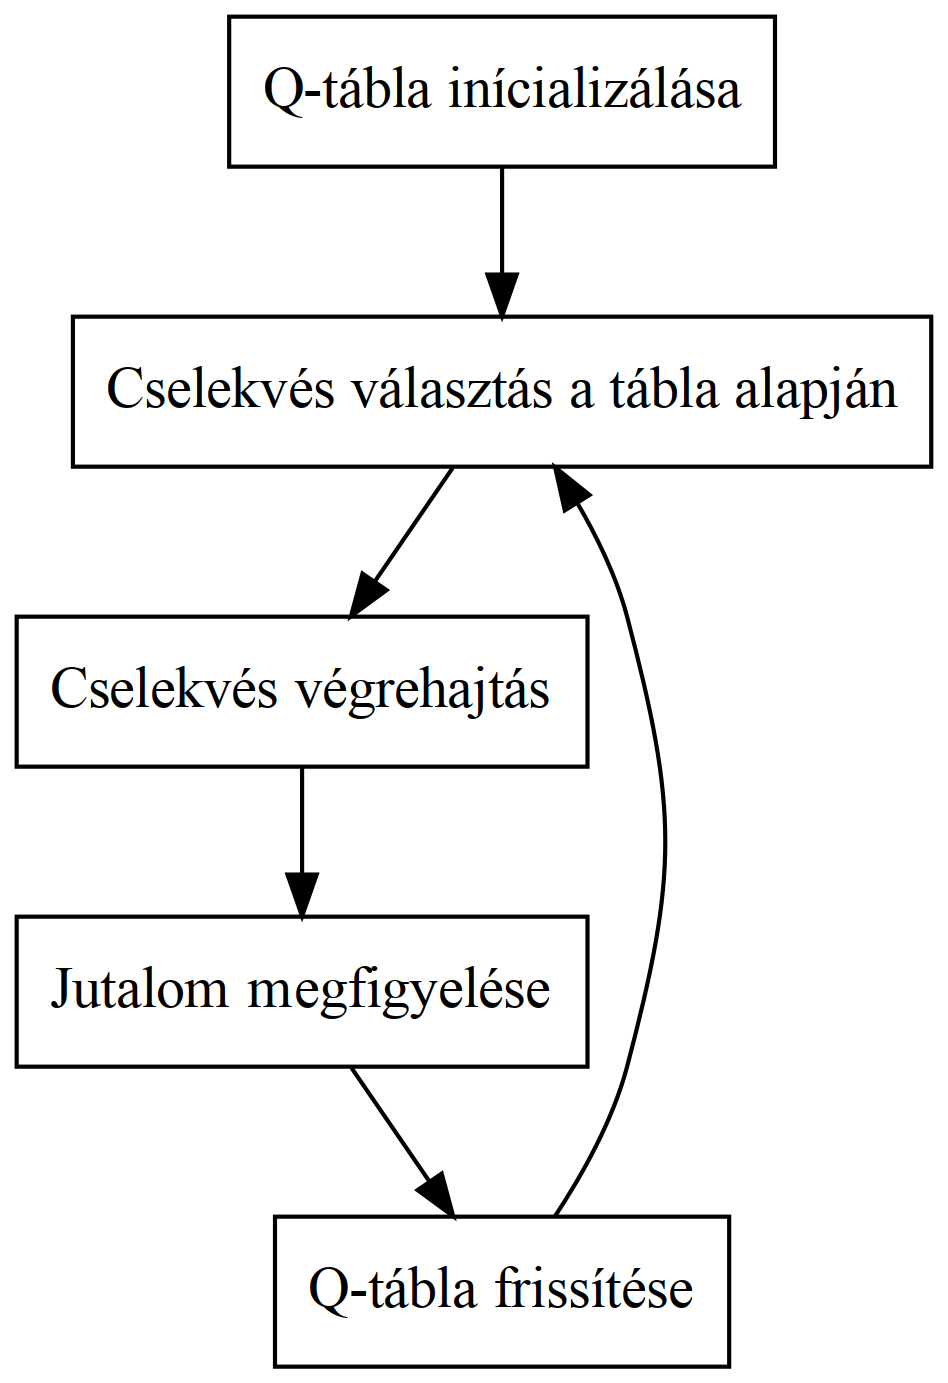
\includegraphics[height=6cm, keepaspectratio]{graphs/ql_1.png}
\end{center}
\end{column}
\begin{column}{.5\textwidth}
\begin{center}
Példa $Q$-táblára\par\medskip
\begin{tabular}{|c|c|c|c|c|}
\hline
& \text{$a_0$} & \text{$a_1$} & \text{$a_2$} & \text{$a_3$} \\
\hline
\text{$s_0$} & $0.76$ & $0.41$ & $0.92$ & $-0.14$ \\
\hline
\text{$s_1$} & $-0.65$ & $0.31$ & $-0.07$ & $0.55$ \\
\hline
\text{$s_2$} &  $0.23$ & $-0.99$ & $0.67$ & $-0.43$ \\
\hline
\text{$s_3$} & $-0.81$ & $0.79$ & $-0.58$ & $0.17$ \\
\hline
\text{$s_4$} & $0.62$ & $-0.28$ & $0.96$ & $-0.72$ \\
\hline
\text{$s_5$} & $-0.36$ & $0.08$ & $-0.51$ & $0.64$ \\
\hline
\end{tabular}
\end{center}
\par\medskip
A $Q$-tábla tárolja el a $Q(s,a)$ értékeket minden $s \in S$ és $a \in A$ párosra. 
\end{column}
\end{columns}
\end{frame}

\begin{frame}{}
\begin{algorithm}[H]
\caption{$Q$-tanulás algoritmusa $\pi \approx \pi_*$ megbecslésére}
\SetAlgoLined
\textbf{Input}: $\alpha$ tanulási sebesség; $\varepsilon > 0$ hibahatár\par
$Q(s,a) \leftarrow random()$ for $s \in S$, $a \in A$\tcc*[t]{$Q$ értékek inícializálása}
$Q(s_T,\cdot) \leftarrow 0$\tcc*[t]{Terminális állapot $0$-ra állítása}
\For{$i=0 \rightarrow max_i$}{
	$s \leftarrow s_0$\tcc*[t]{$s$ inícializálása}
	\While{$s \neq s_T$}{
		$a \leftarrow \pi(s)$\tcc*[t]{Cselekvés választása $\pi$ szerint, pl. $\varepsilon$-mohó}
		$a$ végrehajtása, $r, s'$ megfigyelése\;
		$Q(s,a) \leftarrow Q(s,a) + \alpha \left[ r + \gamma \underset{a'}{max} Q(s',a') - Q(s,a) \right]$\;
		$s \leftarrow s'$\tcc*[t]{$s$ frissítése}
	}
}
\end{algorithm}
A politikát a $Q$-tábla határozza meg.
\end{frame}

\begin{frame}{Dupla $Q$-tanulás}
A kettős tanulás ötlete természetesen kiterjed a teljes MDP algoritmusaira. A $Q$-tanulásban a becsült $Q$-értékek torzítottak lehetnek, ha alacsony a minta számossága, vagy zaj van a rendszerben. Egy módja a $Q$-tanulás regularizálásának, ha egy helyet\textbf{ két $Q$-táblát tart nyilván az algoritmus}, $Q_1$-et és $Q_2$-t.\par\smallskip
A $Q$-tanulással analóg dupla $Q$-tanulás nevű kettős tanulási algoritmus két részre osztja az időlépéseket, \textbf{minden lépésnél egy érmét feldobva}. Ha az érme fejre esik, a frissítés a következő:
\begin{block}{}
\[
Q_1(s,a) \leftarrow Q_1(s,a) + \alpha \left[ r + \gamma Q_2 \left(s', \underset{a'}{argmax} Q_1(s',a')\right) - Q_1(s,a) \right]
\]
\end{block}
Ha az érme pedig írásra esik, akkor ugyanez a frissítés $Q_1$ és $Q_2$ felcserélésével történik, így $Q_2$ frissül. A két közelítő értékfüggvényt teljesen szimmetrikusan kezeli az algoritmus. Például egy $\varepsilon$-mohó politika a dupla tanulás esetében az egyes cselekvési értékbecslések \textbf{átlagára vagy összegére épülhet}.
\end{frame}

\begin{frame}{Dupla $Q$-tanulás eljárása}
\begin{columns}
\begin{column}{.5\textwidth}
Mivel két $Q$ táblát kell nyilván tartania, az algoritmus memóriaigénye megkétszereződik. A becsült értékek viszont jóval torzítatlanabbak lesznek, mint az egyszeres $Q$ tanulás esetében. A lépésenkénti számításigény nem növekszik az extra $Q$-tábla bevonásával.
\end{column}
\begin{column}{.5\textwidth}
\begin{center}
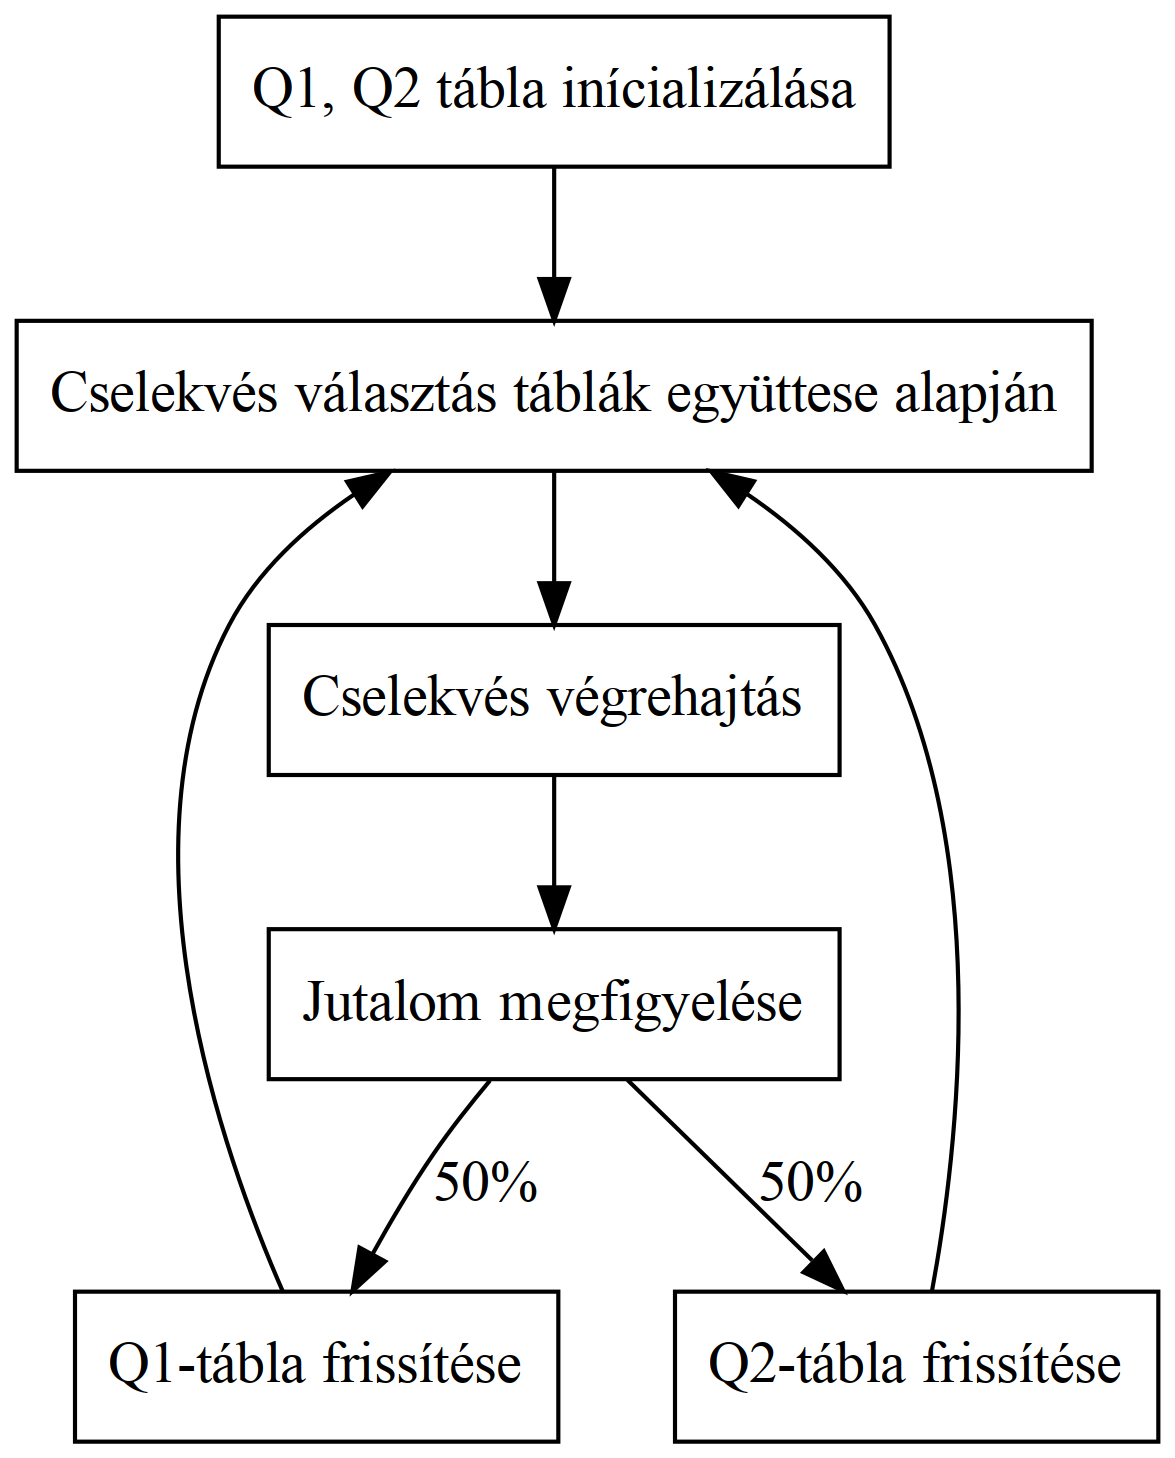
\includegraphics[height=7cm, keepaspectratio]{graphs/ql_2.png}
\end{center}
\end{column}
\end{columns}
\end{frame}

\begin{frame}{}
\begin{algorithm}[H]
\caption{Dupla $Q$-tanulás algoritmusa}
\SetAlgoLined
\begin{small}
\textbf{Input}: $\alpha$ tanulási sebesség; $\varepsilon > 0$ hibahatár\par
$Q_1(s,a) \leftarrow random()$, $Q_2(s,a) \leftarrow random()$ for $s \in S$, $a \in A$\;
$Q_1(s_T,\cdot) \leftarrow 0$, $Q_2(s_T,\cdot) \leftarrow 0$\tcc*[t]{Terminális állapotok $0$-ra állítása}
\For{$i=0 \rightarrow max_i$}{
	$s$ inícializálása\;
	\While{$s \neq s_T$}{
		$a \leftarrow \pi(s)$\tcc*[t]{Cselekvés választása $\pi$ szerint, pl. $\varepsilon$-mohó}
		$a$ végrehajtása, $r$ és $s'$ megfigyelése\;
		\eIf{$p > 0.5$}{
			 $Q_1(s,a) \leftarrow Q_1(s,a) + \alpha \left[ r + \gamma Q_2\left(s', \underset{a'}{argmax} Q_1(s',a')\right) - Q_1(s,a) \right]$
		}{
			$Q_2(s,a) \leftarrow Q_2(s,a) + \alpha \left[ r + \gamma Q_1\left(s', \underset{a'}{argmax} Q_2(s',a')\right) - Q_2(s, a) \right]$
		}
		$s \leftarrow s'$\tcc*[t]{$s$ frissítése}
	}
}
\end{small}
\end{algorithm}
\end{frame}

\section{Függvény illesztés}

\begin{frame}{}
\tableofcontents[currentsection]
\end{frame}

\begin{frame}{Függvény illesztés alapjai}
\begin{columns}
\begin{column}{.5\textwidth}
A függvény illesztés eljárása szerint valamely $x$ \textbf{független változóból} vett minta alapján szeretnénk előre jelezni egy $y$ \textbf{függő változó} értékét azért, hogy feltárja az adatpontok közötti mintázatokat.\par\smallskip
Két eljárása ismert:
\begin{itemize}
	\item \textbf{Regresszió}: tárgya egy folytonos változó
	\item \textbf{Osztályozás}: tárgya egy diszkrét változó
\end{itemize}
A függvény illesztés eredménye a \textbf{modell}.
\end{column}
\begin{column}{.5\textwidth}
\begin{center}
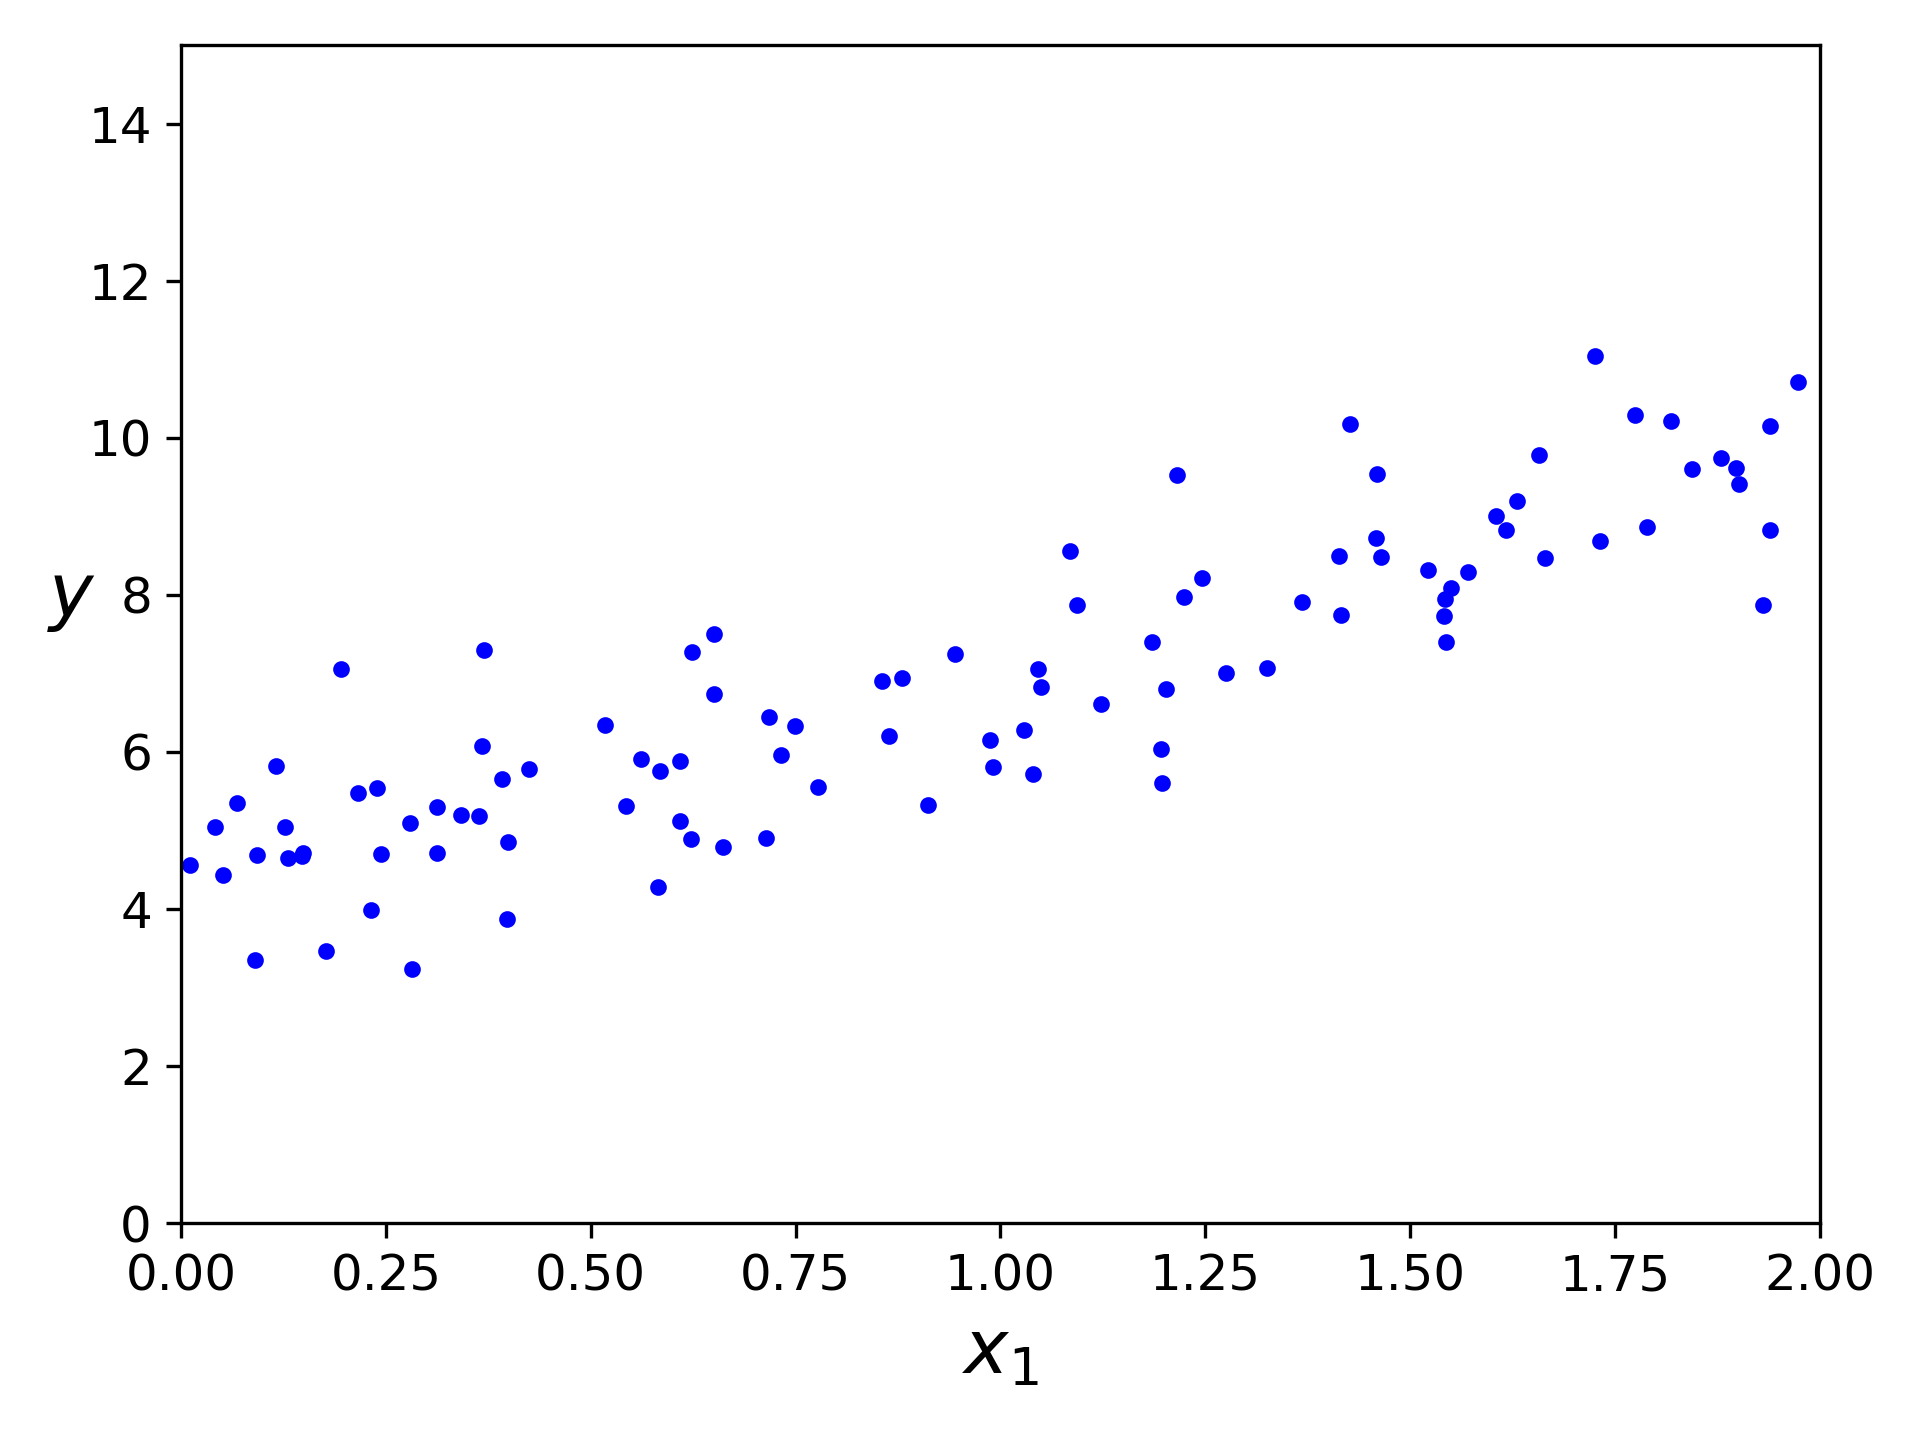
\includegraphics[width=7cm, keepaspectratio]{images/ql_8.png}
\end{center}
\end{column}
\end{columns}
\end{frame}

\begin{frame}{Függvény illesztés alapjai}
\begin{columns}
\begin{column}{.5\textwidth}
Az illesztett modell alakját és viselkedését a \textbf{paraméterei} határozzák meg, amelyek együtthatókként viselkednek a modell egyenletében. A lineáris modell egyenlete: 
\begin{block}{}
\vspace{-0.25cm}
\[
y_i = \theta_0 + \theta_1x_i + \varepsilon_i
\]
\end{block}
Ahol:
\begin{itemize}
	\item $\theta_0$: az $y$ tengely metszéspontja, vagy eltolás
	\item $\theta_1$: az egyenes meredeksége
	\item $\varepsilon$: a véletlen hiba, amit a modell nem tud előre jelezni
\end{itemize}
$\theta=[\theta_0,\theta_1,...,\theta_n]$ a paraméterek vektora.
\end{column}
\begin{column}{.5\textwidth}
\begin{center}
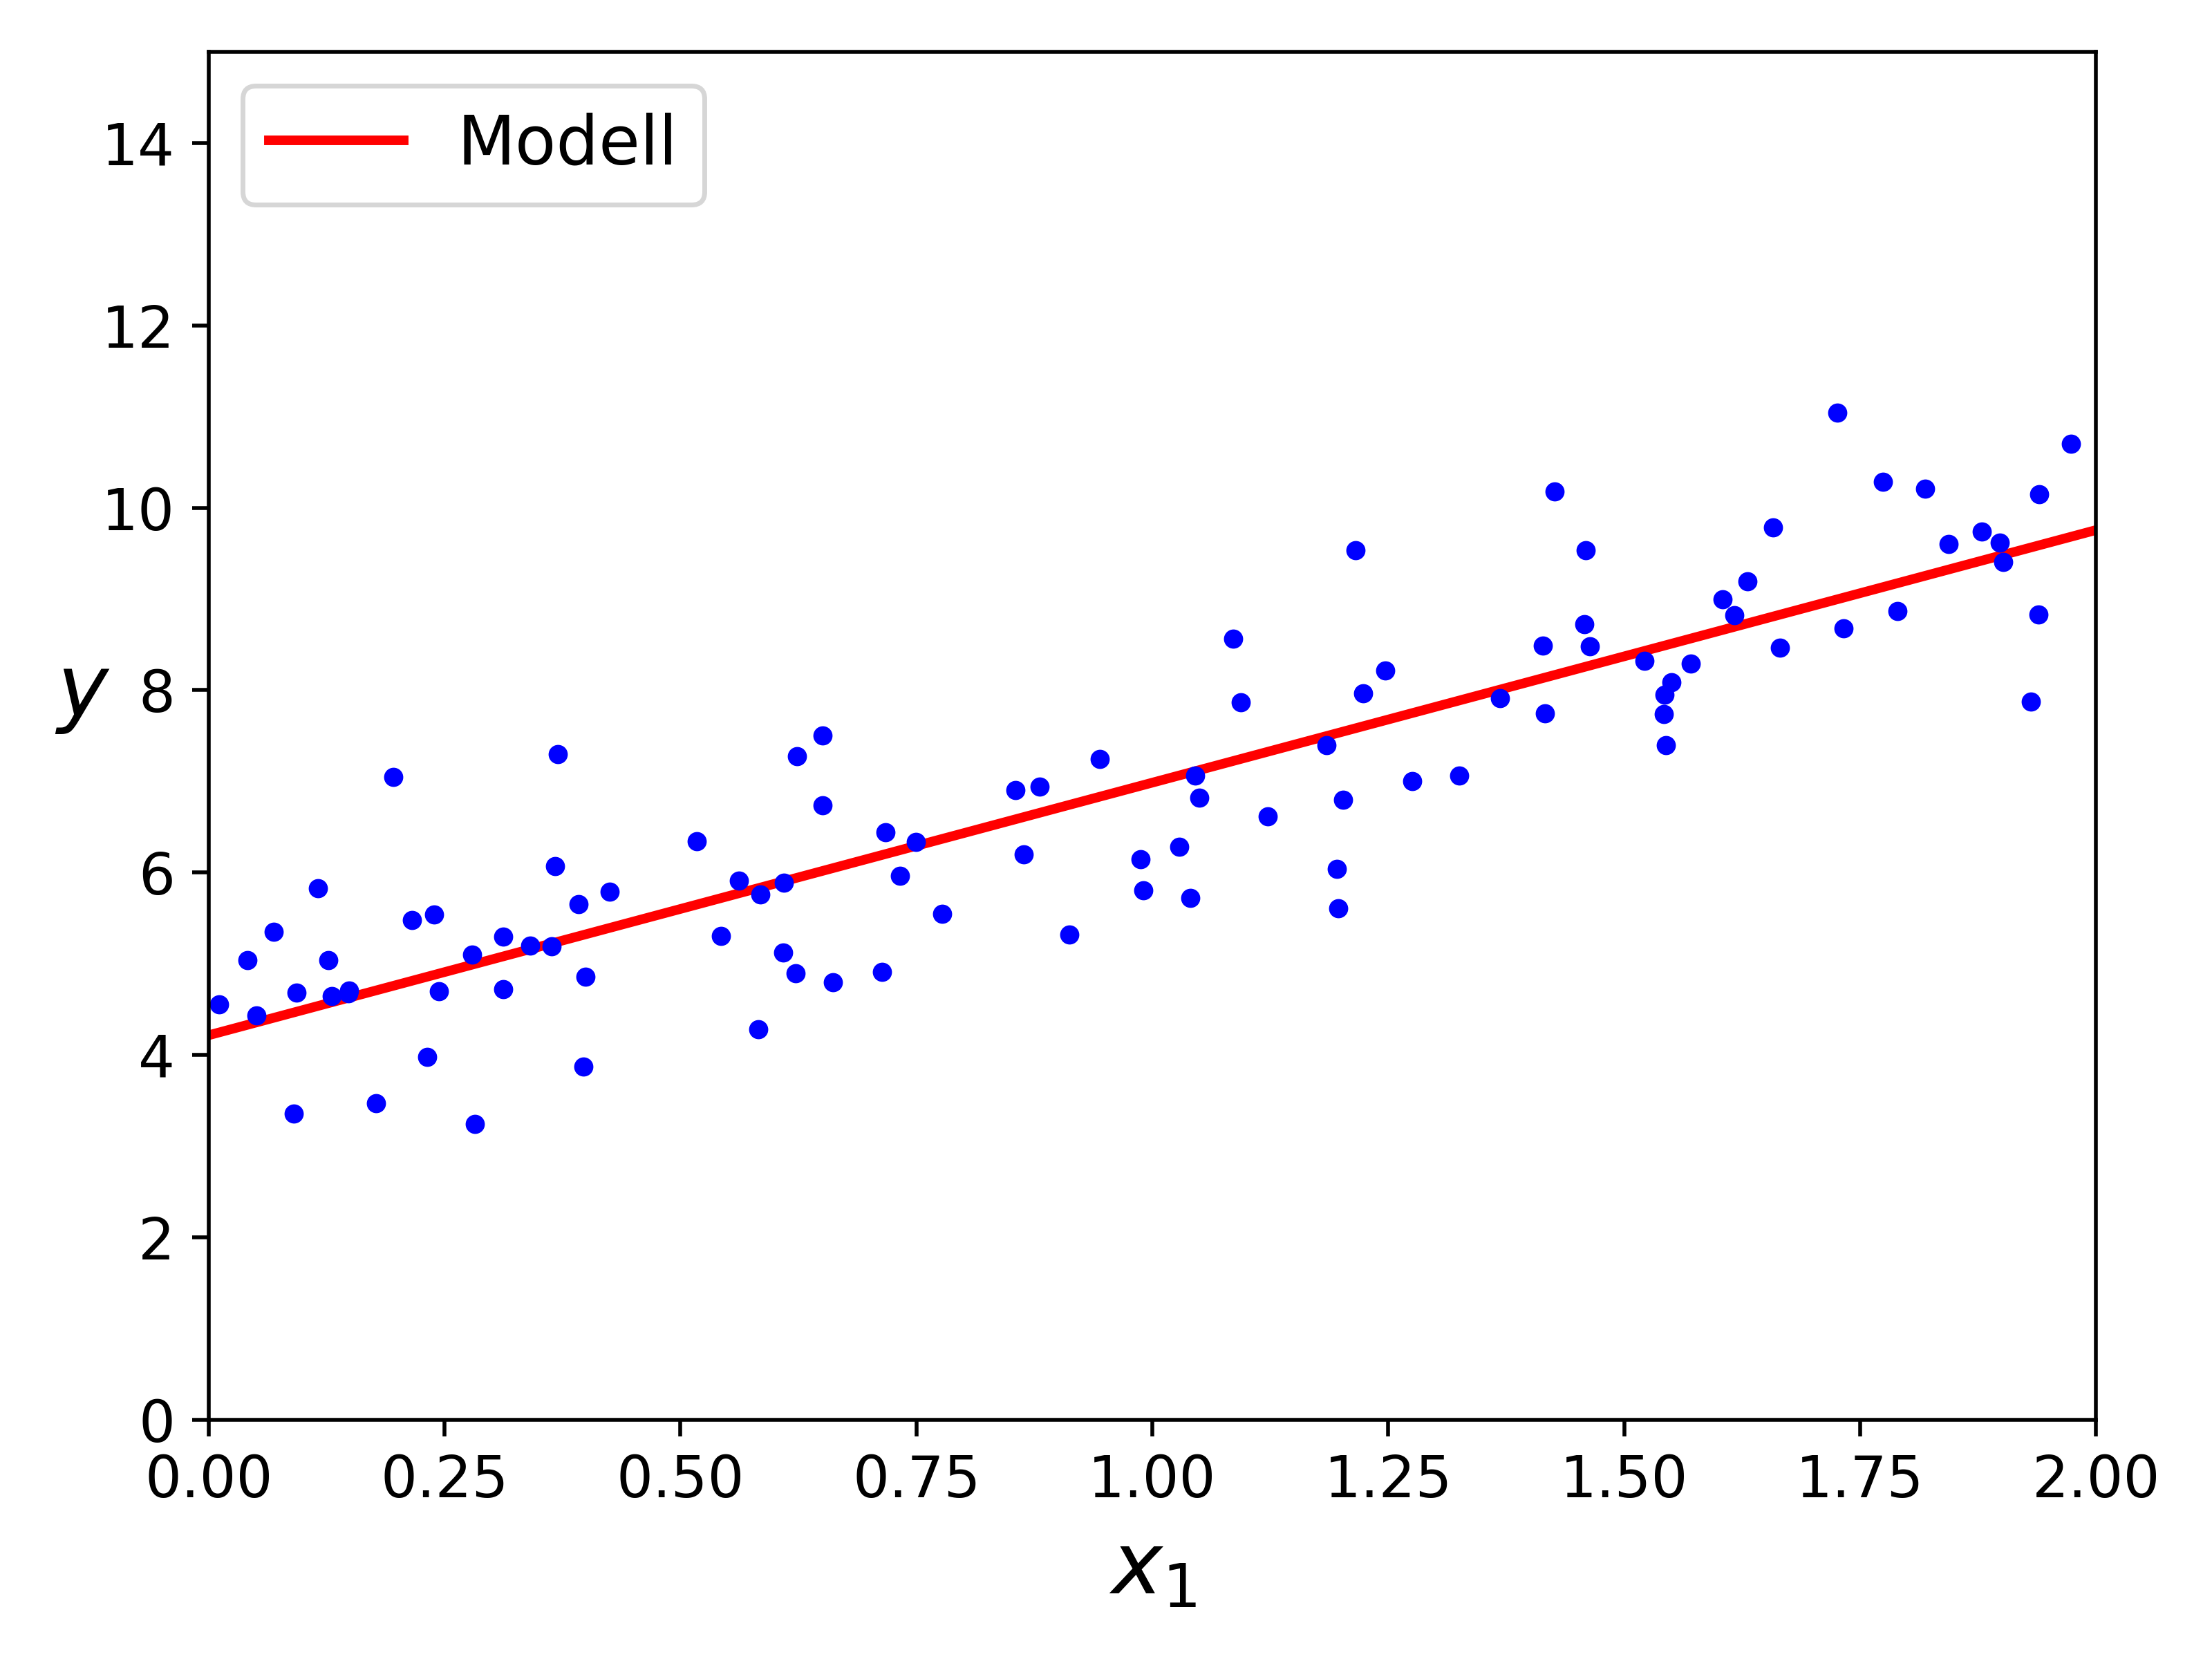
\includegraphics[width=7cm, keepaspectratio]{images/ql_9.png}
\end{center}
\end{column}
\end{columns}
\end{frame}

\begin{frame}{Függvény illesztés több paraméterrel}
\begin{columns}
\begin{column}{.5\textwidth}
Függvényt lehetséges nemlineáris adatokra is illeszteni. Ebben a példában a minta adatpontok kvadratikusak, \textbf{nem írhatók le egy lineáris egyenlettel}. A modellnek ebben az esetben $3$ paramétere van: $\theta_0$, $\theta_1$ és $\theta_2$. Az illesztett modell egyenlete: 
\[
y=1.78 + 0.93x + 0.56 x^2
\]
Tehát ebben az esetben $\theta_0=1.78$, $\theta_1=0.93$ és $\theta_2=0.56$.
\end{column}
\begin{column}{.5\textwidth}
\begin{center}
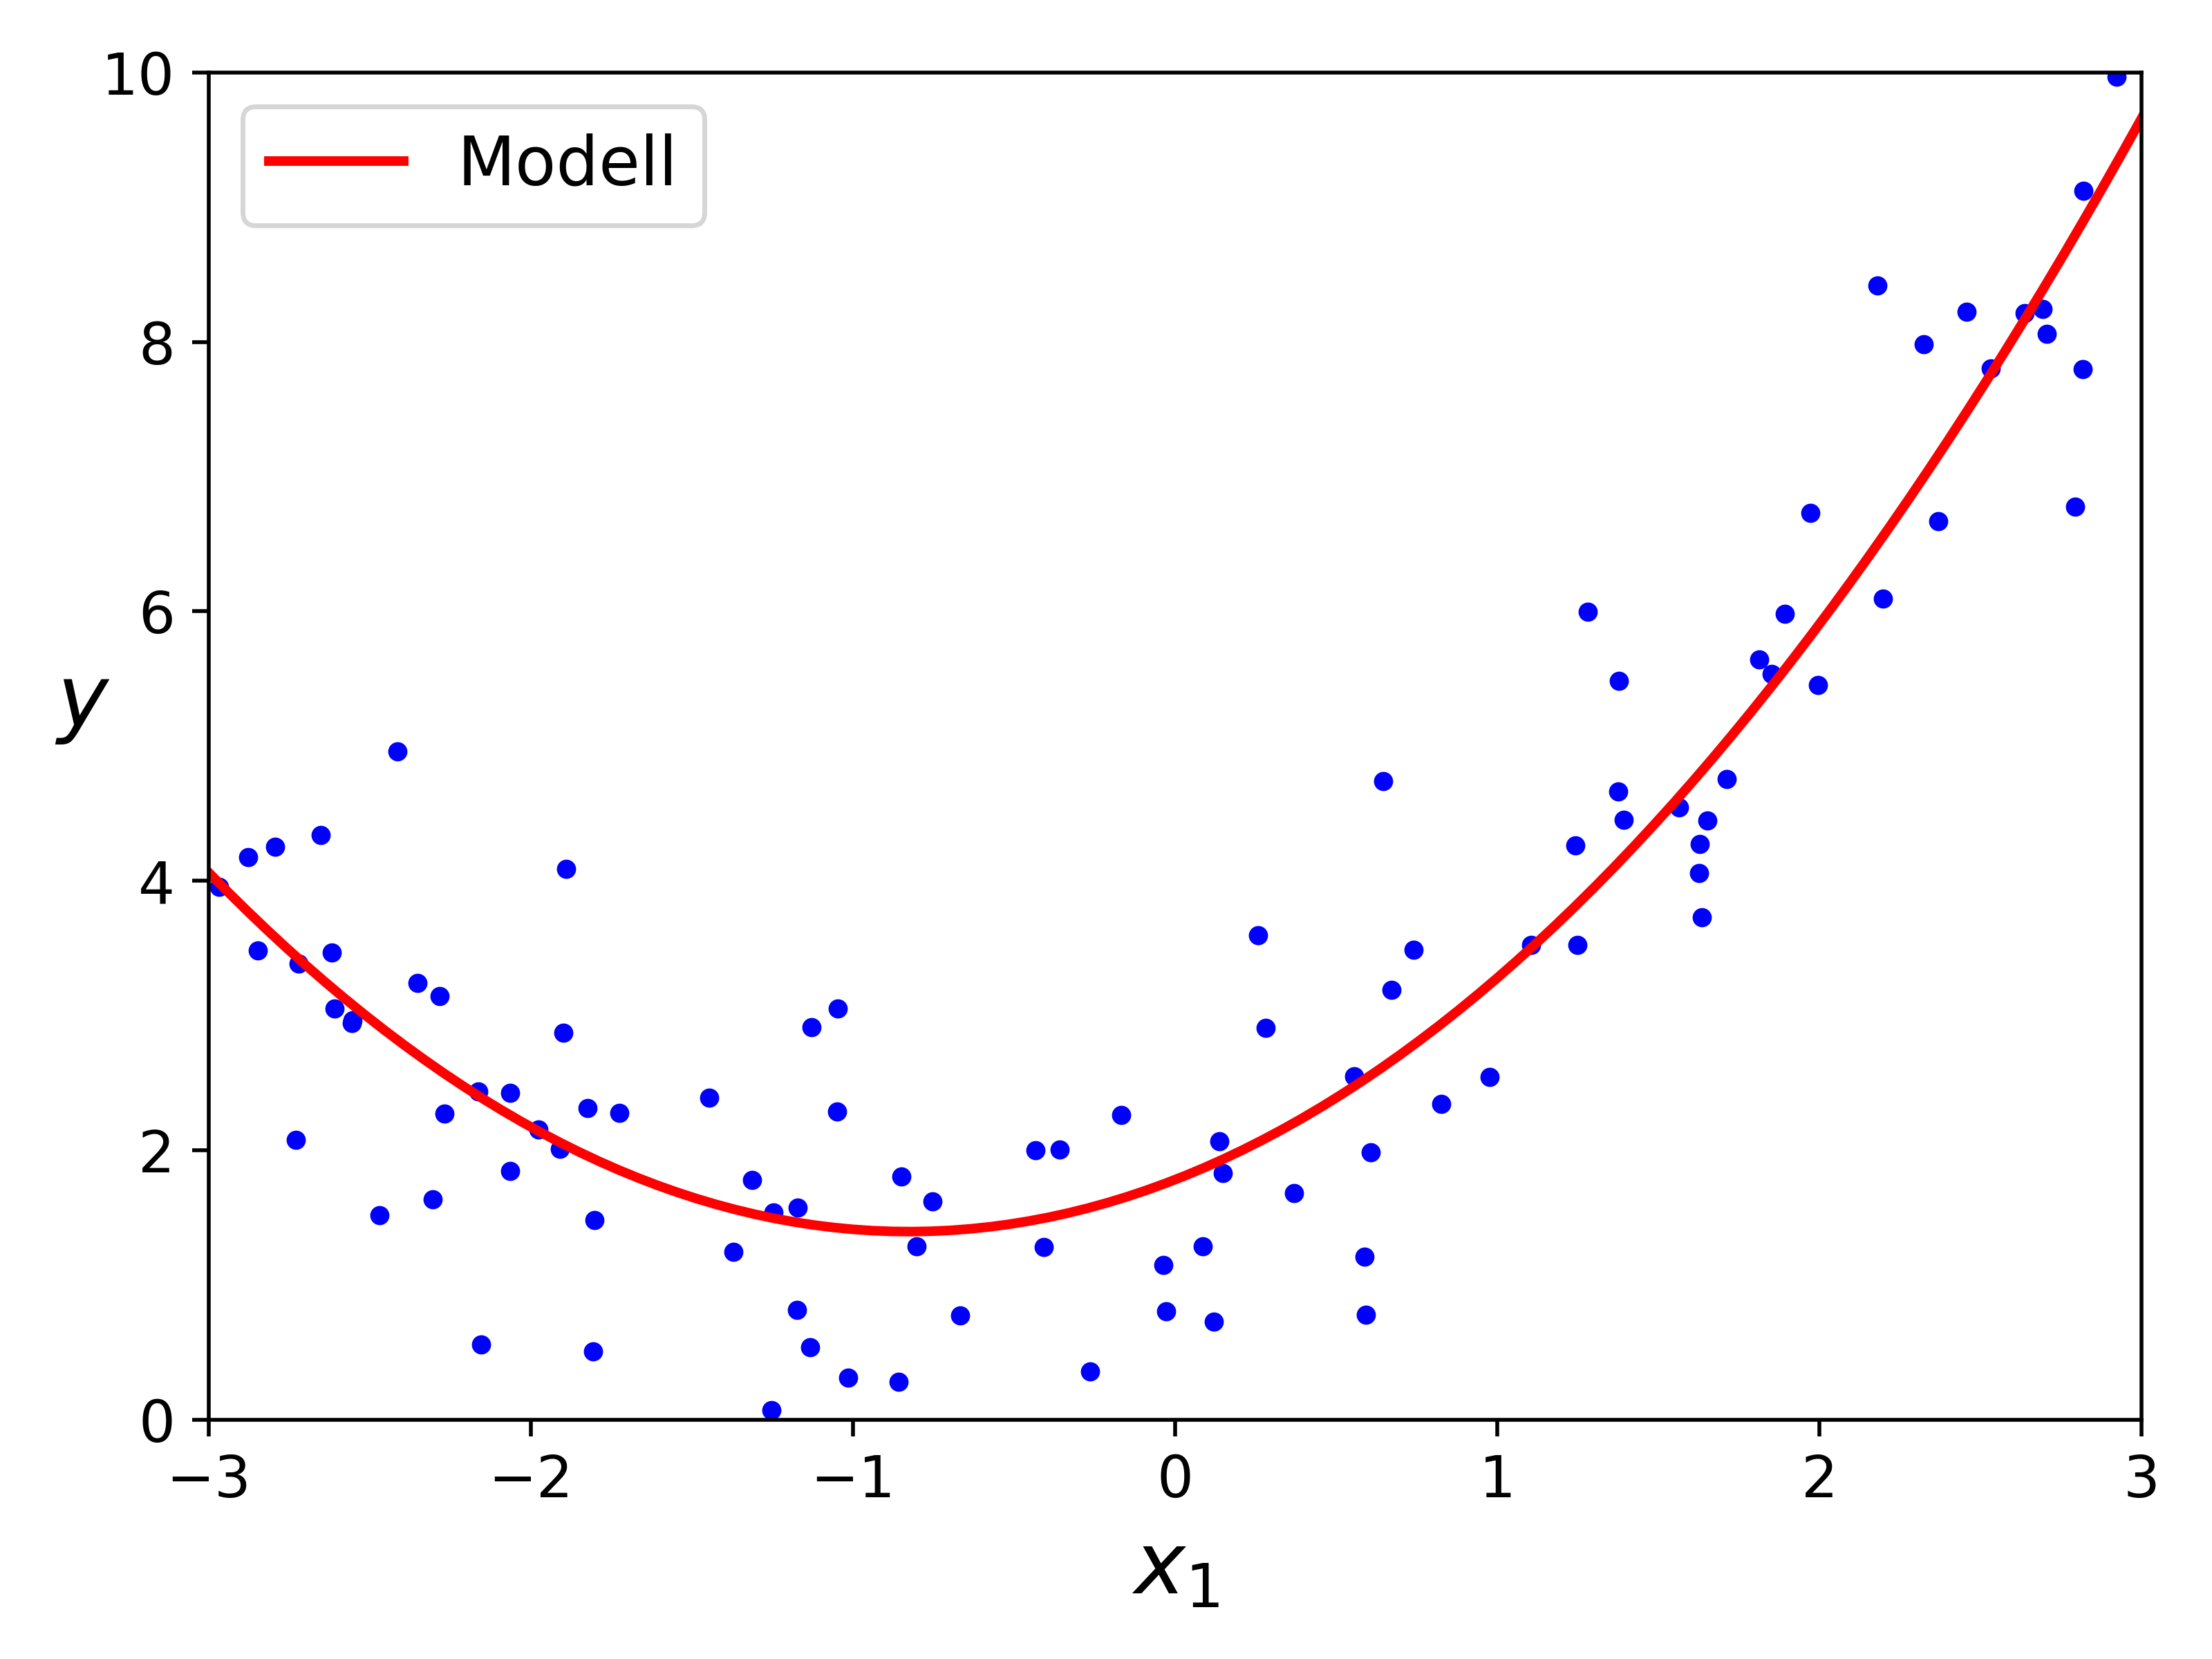
\includegraphics[width=7cm, keepaspectratio]{images/ql_10.png}
\end{center}
\end{column}
\end{columns}
\end{frame}

\section{Gradiens ereszkedés}

\begin{frame}
\tableofcontents[currentsection]
\end{frame}

\begin{frame}{A költségfüggvény}
\begin{columns}
\begin{column}{.5\textwidth}
A modell illesztő algoritmusok mindegyike úgy találja meg az optimális függvényt, hogy valamilyen költségfüggvényt minimalizál. A leggyakoribb ilyen költségfüggvény az \textbf{átlagos négyzetes hiba}:
\begin{block}{}
\[
MSE = \frac{1}{n} \sum_{i=1}^n \left( y_i - f(x)_i \right) 
\]
\begin{itemize}
	\item $y_i$: Megfigyelt adatpont
	\item $f(x)_i$: Modell által adott becslés
\end{itemize}
\end{block}
\end{column}
\begin{column}{.5\textwidth}
\begin{center}
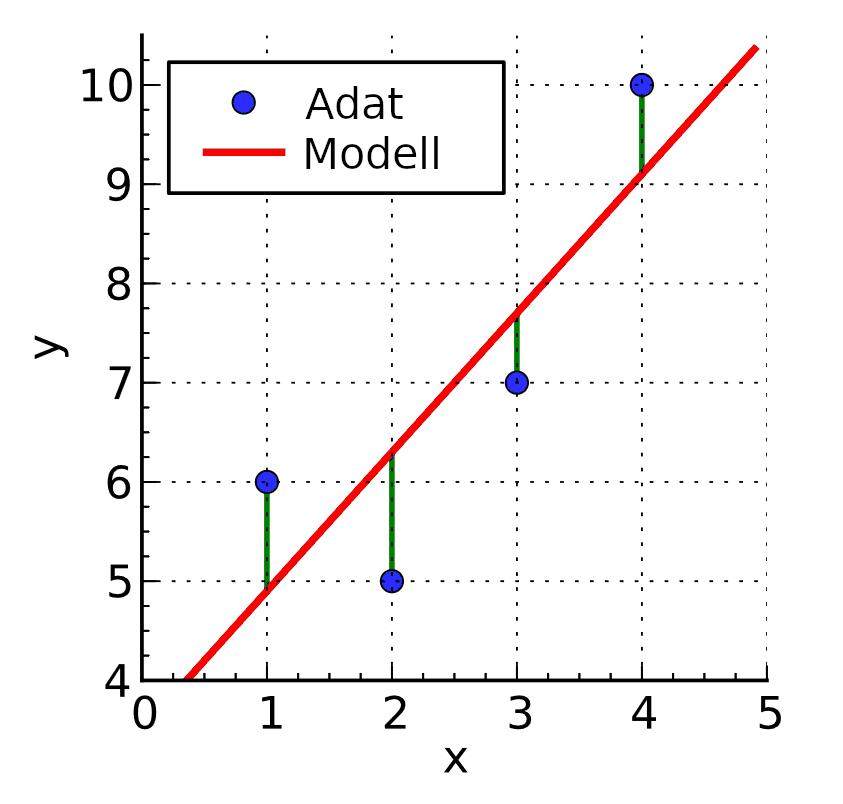
\includegraphics[width=6cm, keepaspectratio]{images/ql_11.png}
\end{center}
\end{column}
\end{columns}
\end{frame}

\begin{frame}{A gradiens}
\begin{columns}
\begin{column}{.5\textwidth}
A függvény illesztés célja, hogy megtalálja azt a modellt, ami a legjobban illeszkedik az adatpontokra, tehát \textbf{minimalizálja a költségfüggvényt} (MSE). 
\begin{block}{Gradiens}
Olyan vektor, amely megmutatja hogyan változik a függvény, és megadja a legnagyobb változás irányát minden dimenzióban.
\vspace{-0.25cm}
\[
df = \nabla f * dx
\]
\end{block} 
A gradiens segítségével meg lehet határozni, merre és mennyivel érdemes változtatni a paramétereket a célfüggvény értékének csökkentése érdekében.
\end{column}
\begin{column}{.5\textwidth}
\begin{center}
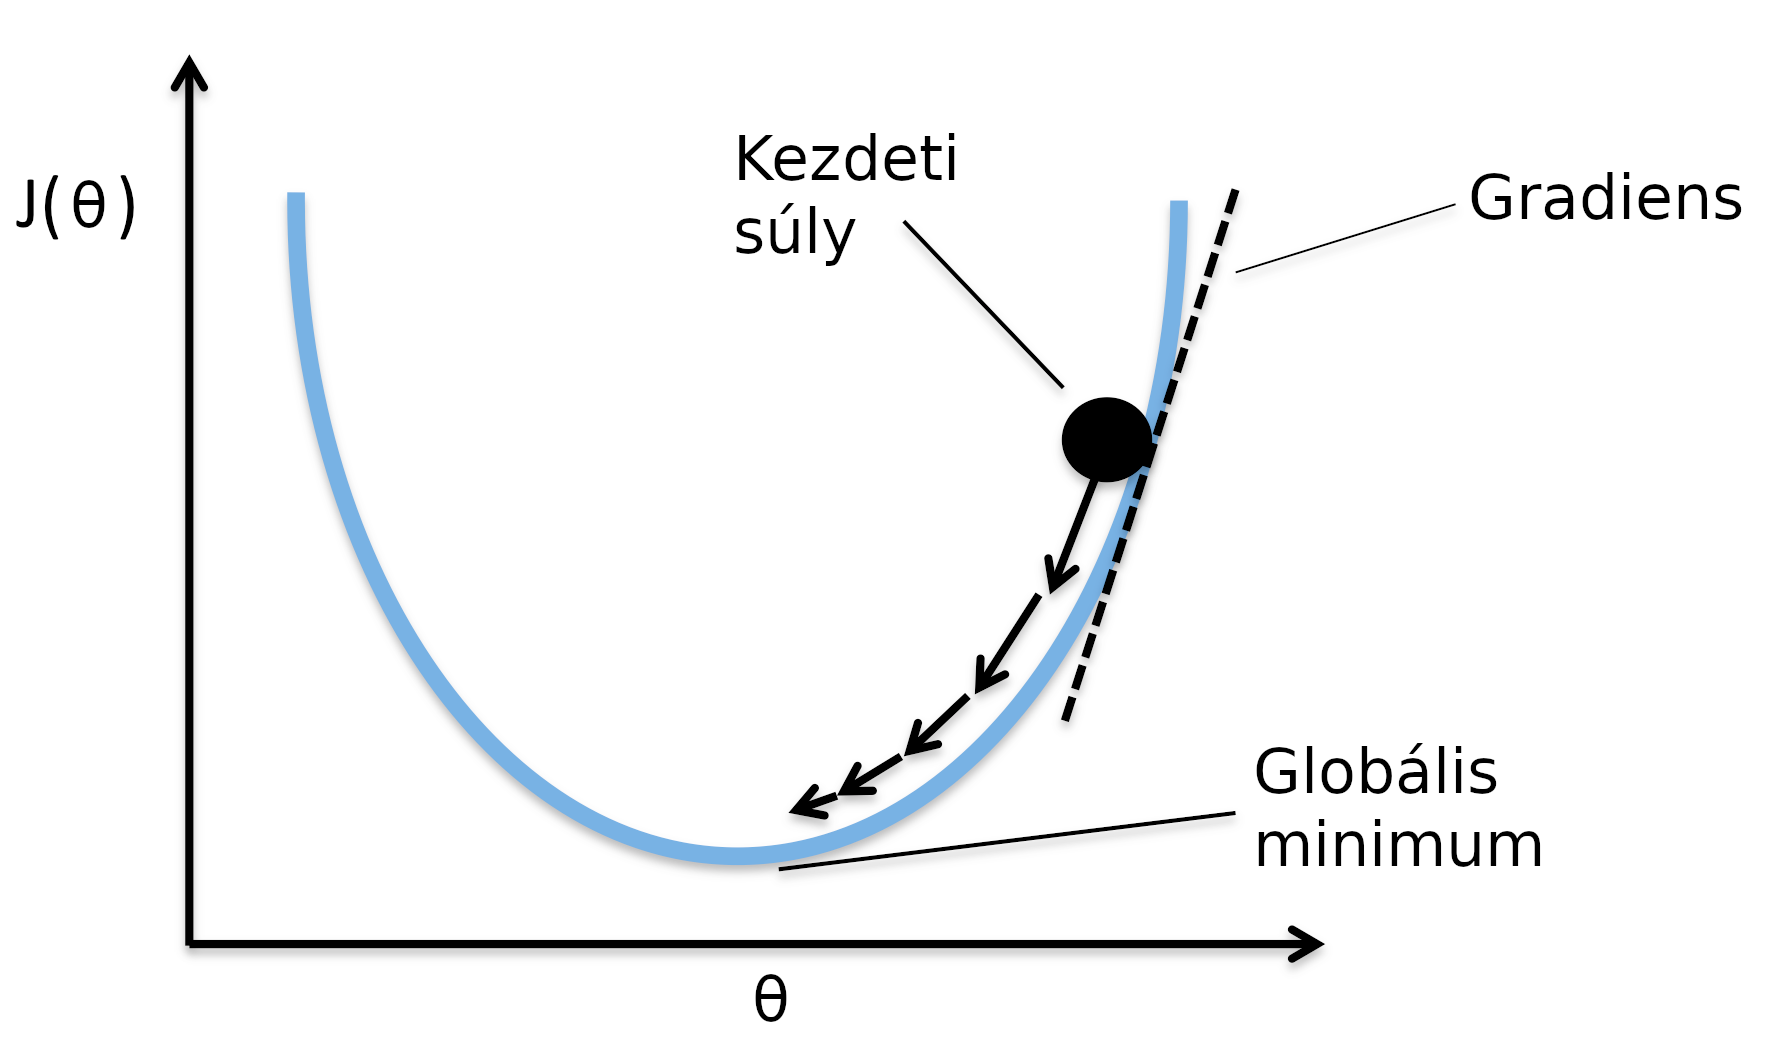
\includegraphics[width=7.5cm, keepaspectratio]{images/ql_12.png}
\end{center}
\end{column}
\end{columns}
\end{frame}

\begin{frame}{Gradiens ereszkedés}
\begin{columns}
\begin{column}{.5\textwidth}
\only<1>{A gradiens ereszkedés egy iteratív minimalizálási algoritmus egy tetszőleges függvény lokális minimum helyének megtalálására. Az algoritmus lépésről lépésre mozog a függvény értékének csökkentése érdekében. \par\smallskip
\begin{block}{Tanulási sebesség ($\alpha$ vagy $\eta$)}
A tanulási sebesség meghatározza, mennyire nagy lépéseket tesz a gradiens ereszkedés az optimalizációs folyamat során.
\end{block}}
\only<2>{\begin{block}{A gradiens ereszkedés paraméter frissítése:}
\[
\theta' \leftarrow \theta - \alpha \; \nabla_\theta \; J(\theta)
\]
\begin{itemize}
	\item $\theta=[\theta_0,\theta_1,...,\theta_n]$: Paraméterek vektora
	\item $\alpha \in [0,1]$: Tanulási sebesség
	\item $\nabla_\theta$: Költségfüggvény gradiense \\($\theta$ szerinti derivált)
	\item $J(\theta)$: Költségfüggvény $\theta$ szerint \\(pl. MSE)
\end{itemize}
\end{block}}
\end{column}
\begin{column}{.5\textwidth}
\only<1>{\begin{center}
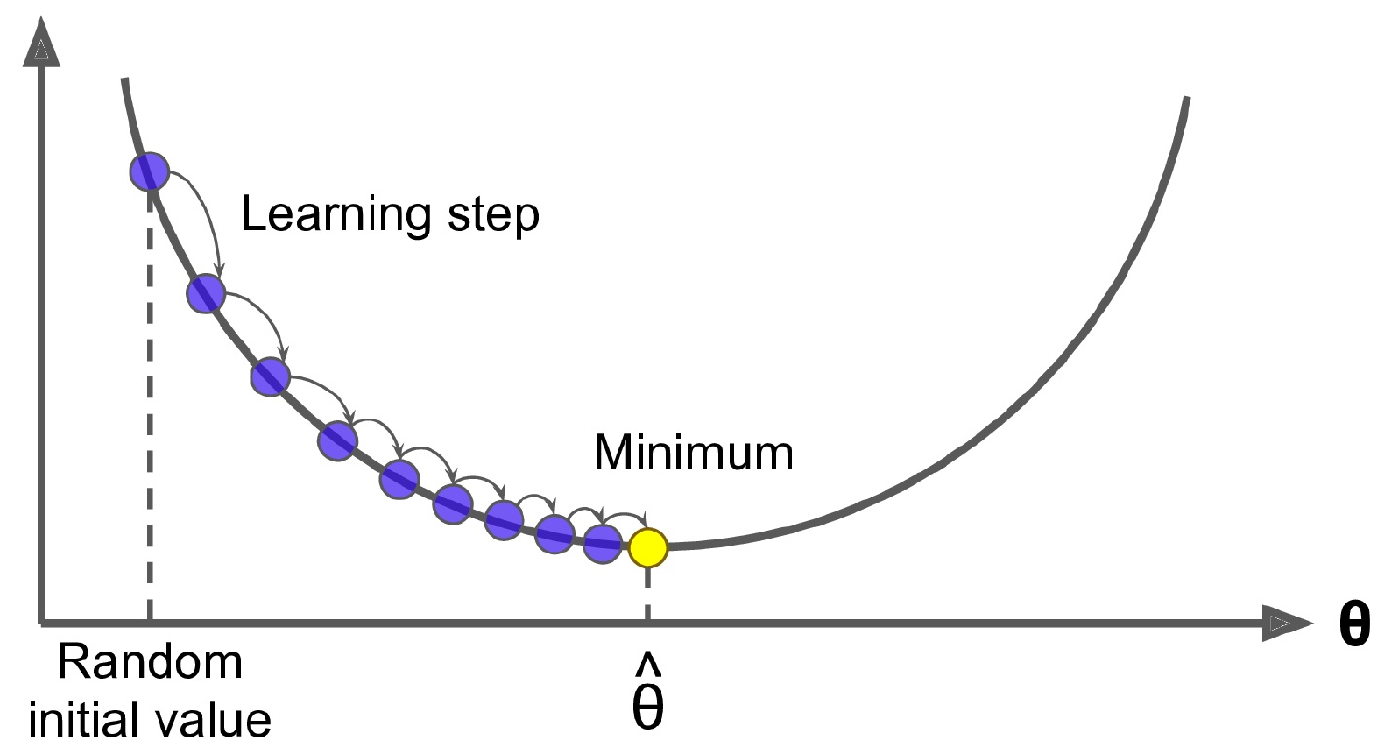
\includegraphics[width=7cm, keepaspectratio]{images/ql_13.png}
\end{center}}
\only<2>{\begin{center}
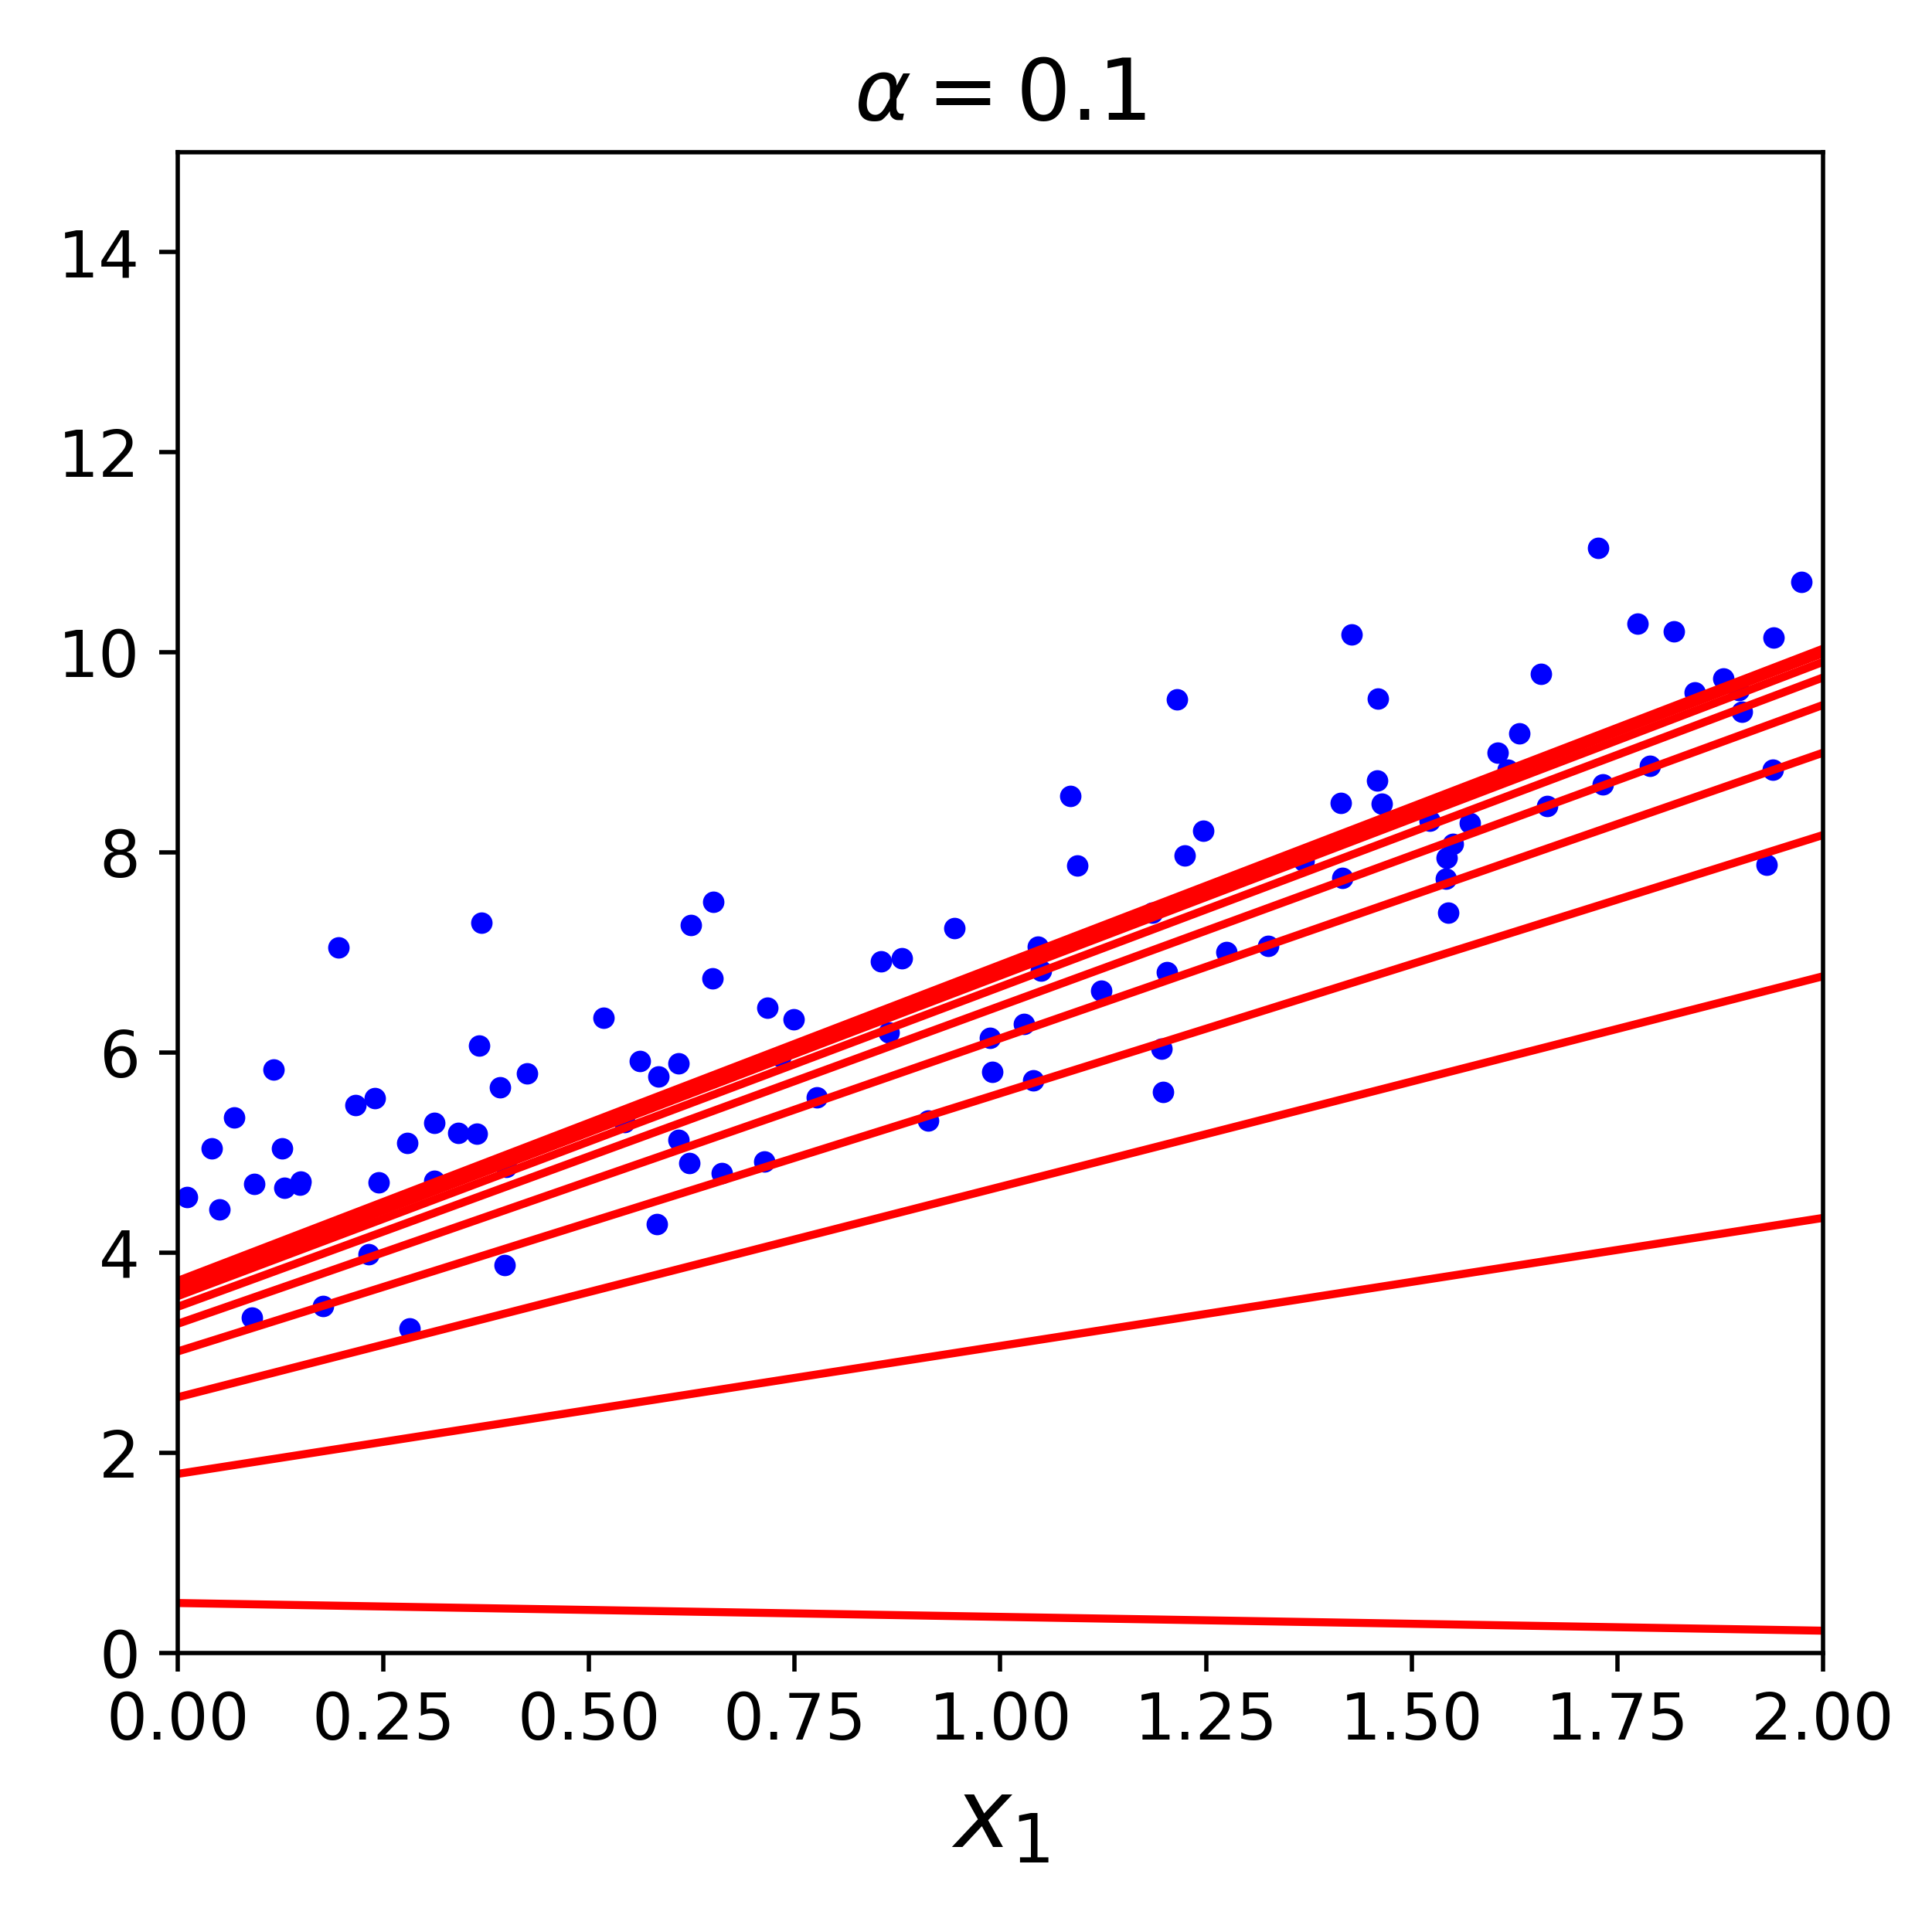
\includegraphics[width=7cm, keepaspectratio]{images/ql_20.png}
\end{center}}
\end{column}
\end{columns}
\end{frame}

\begin{frame}{Túl alacsony tanulási sebesség}
\begin{columns}
\begin{column}{.5\textwidth}
\begin{center}
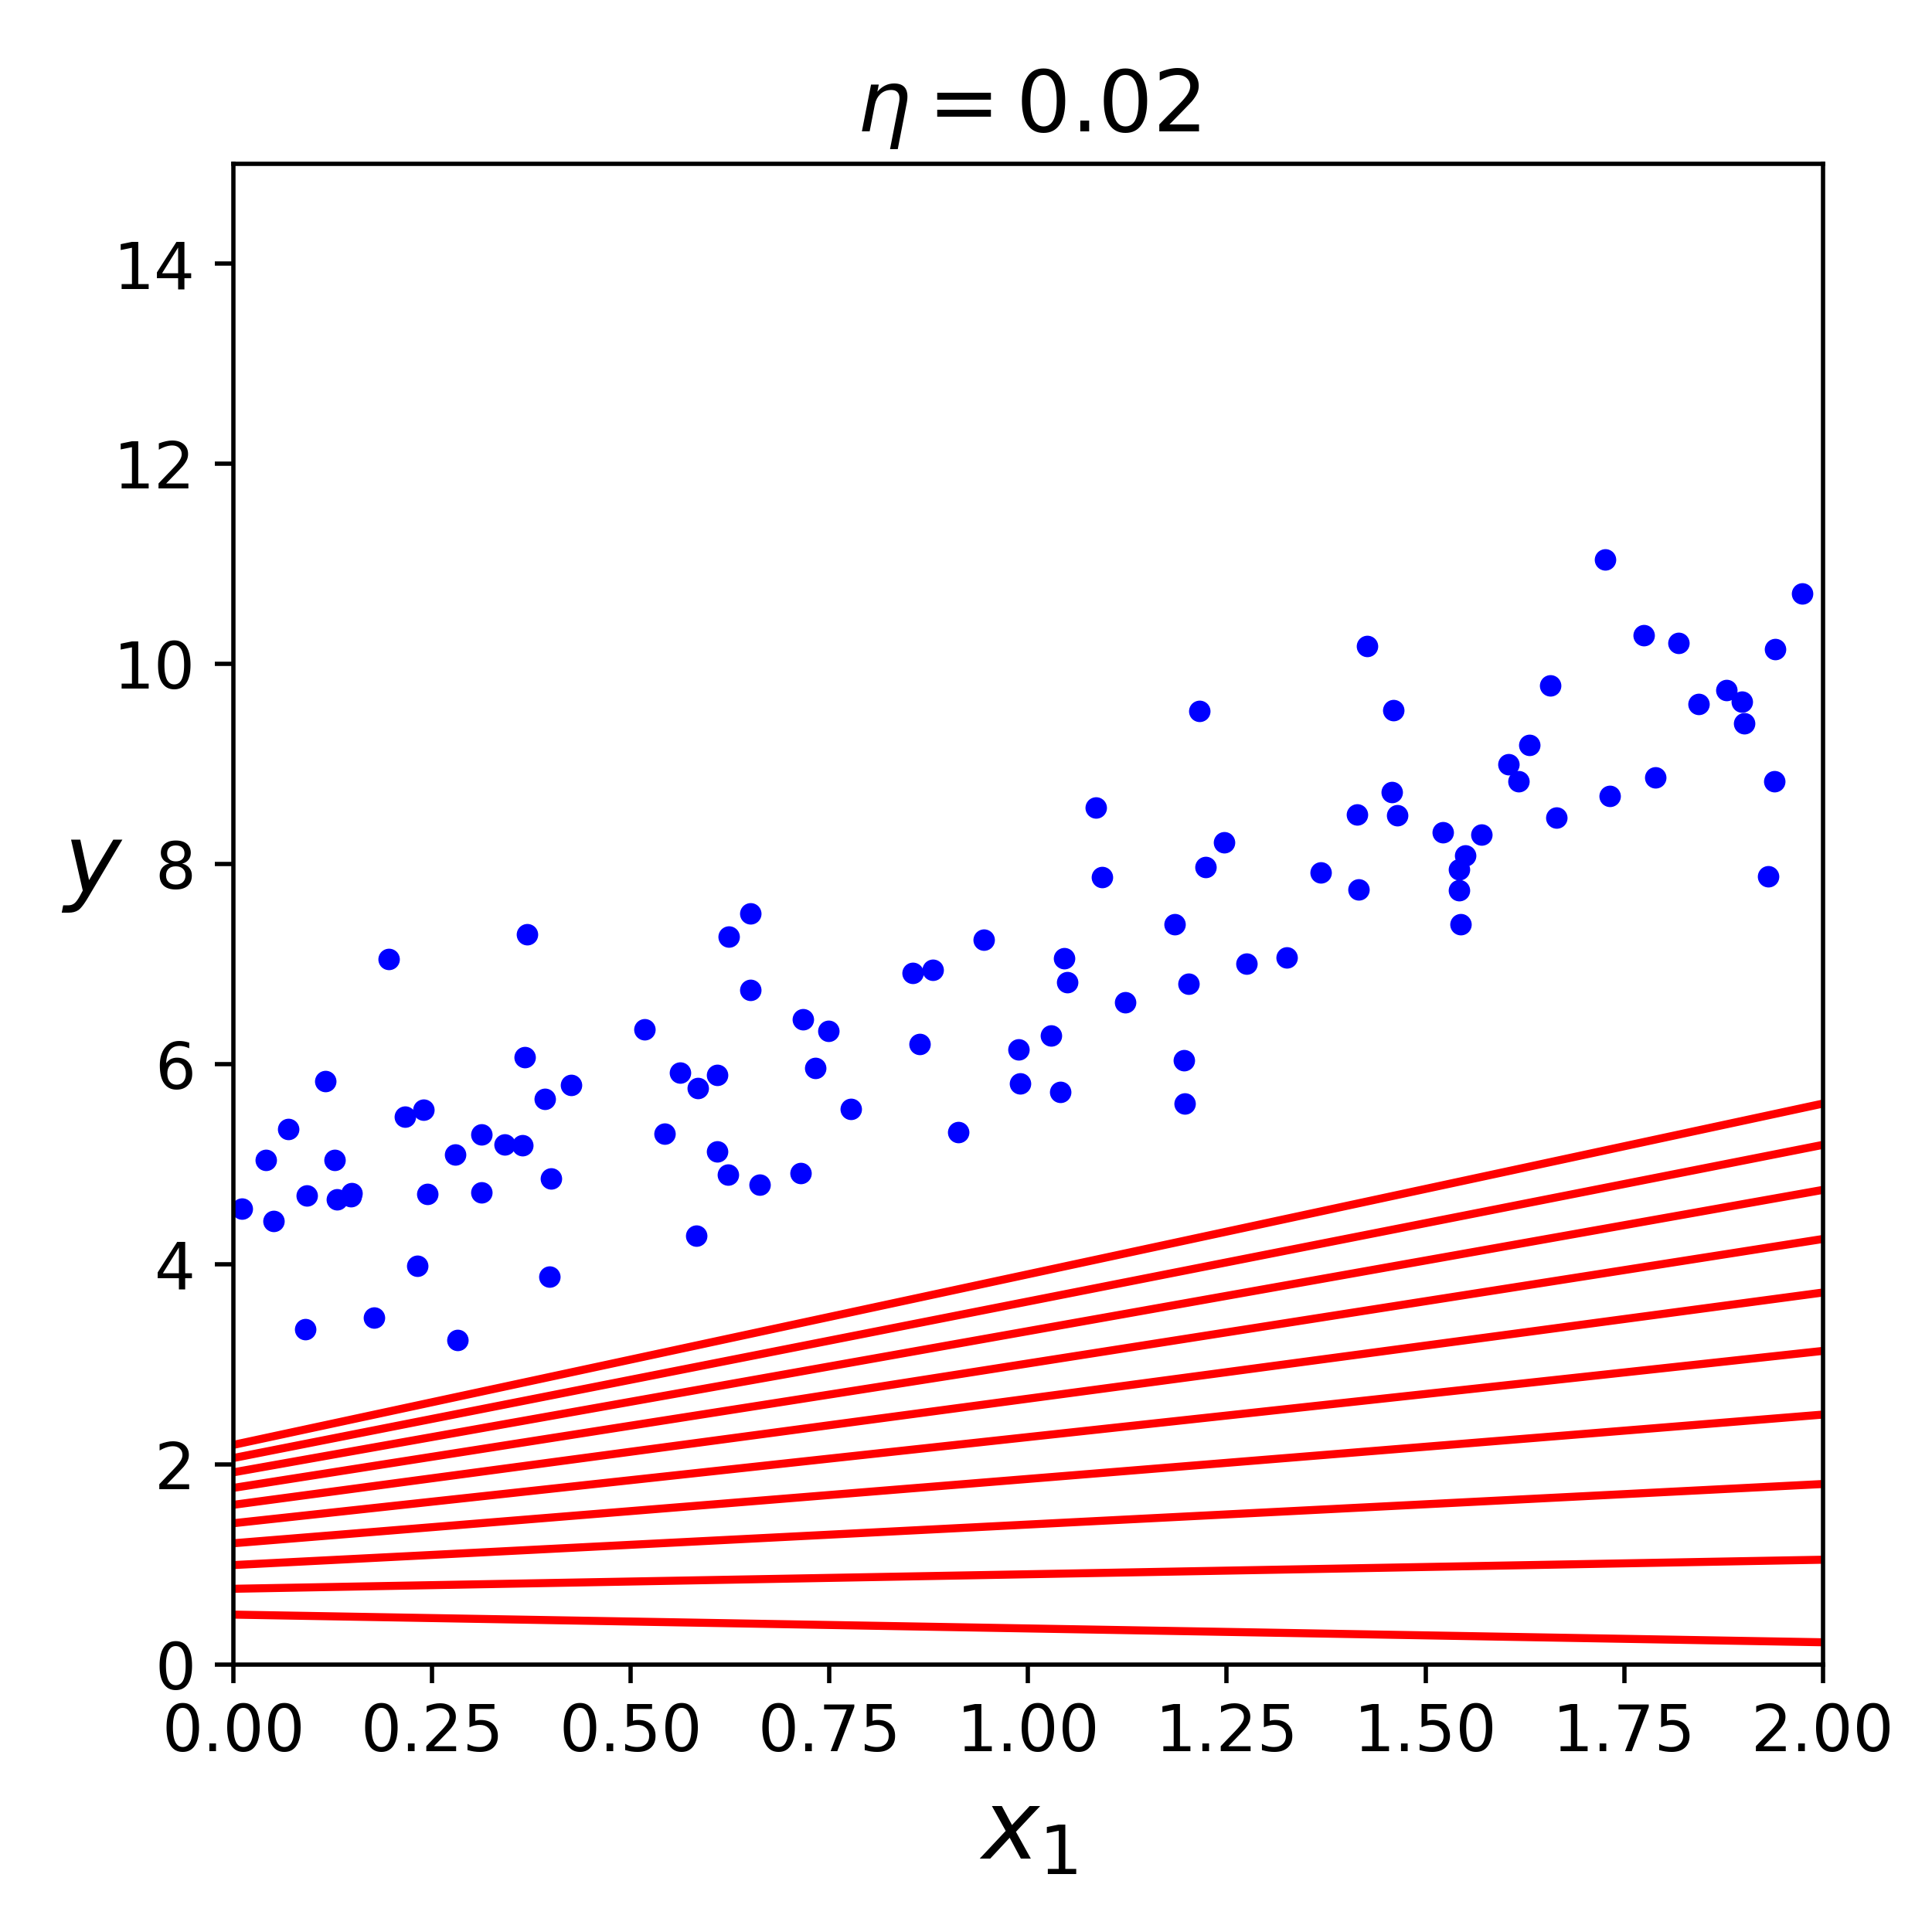
\includegraphics[width=6cm, keepaspectratio]{images/ql_17.png}
\end{center}
\end{column}
\begin{column}{.5\textwidth}
\begin{center}
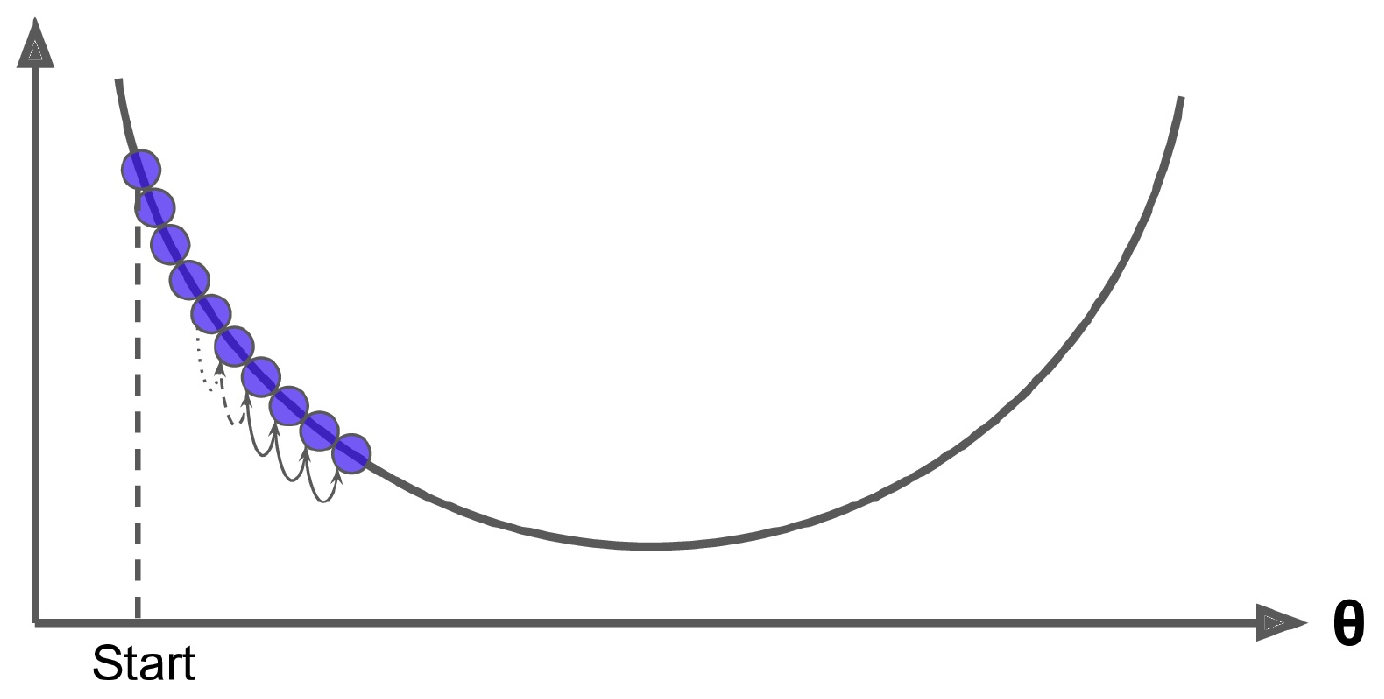
\includegraphics[width=7cm, keepaspectratio]{images/ql_14.png}
\end{center}
\end{column}
\end{columns}
\end{frame}

\begin{frame}{Túl magas tanulási sebesség}
\begin{columns}
\begin{column}{.5\textwidth}
\begin{center}
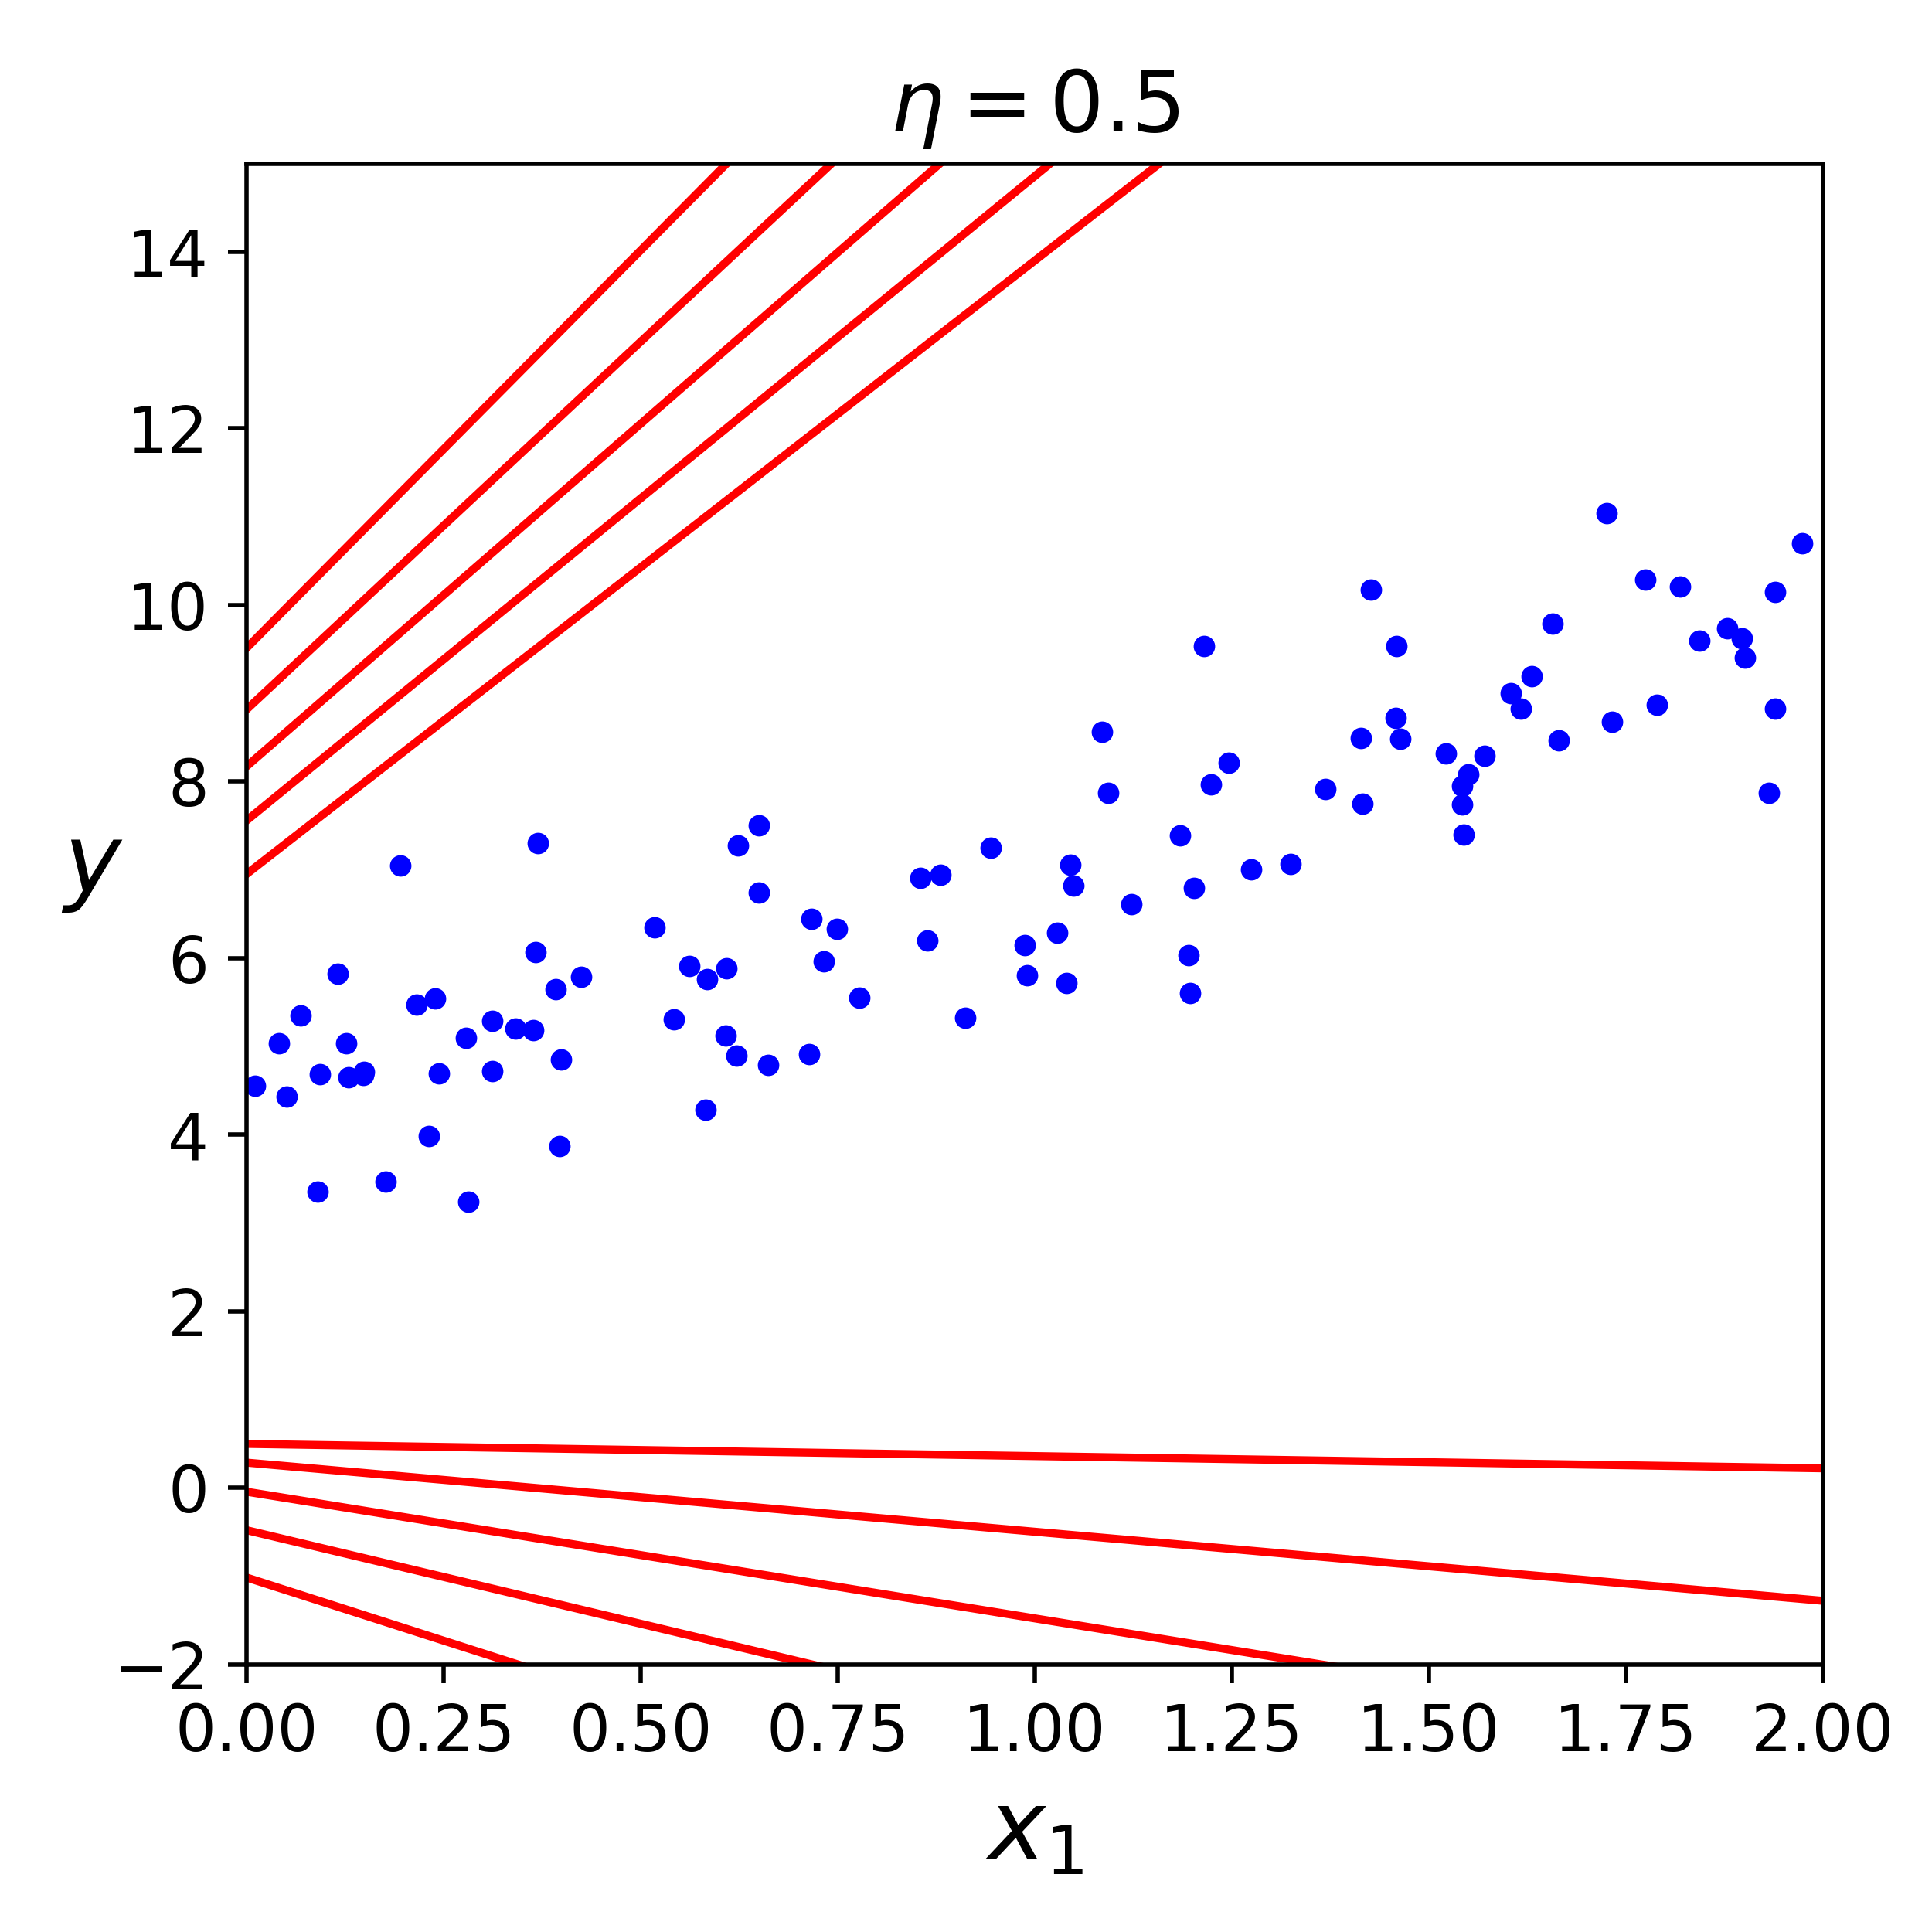
\includegraphics[width=6cm, keepaspectratio]{images/ql_19.png}
\end{center}
\end{column}
\begin{column}{.5\textwidth}
\begin{center}
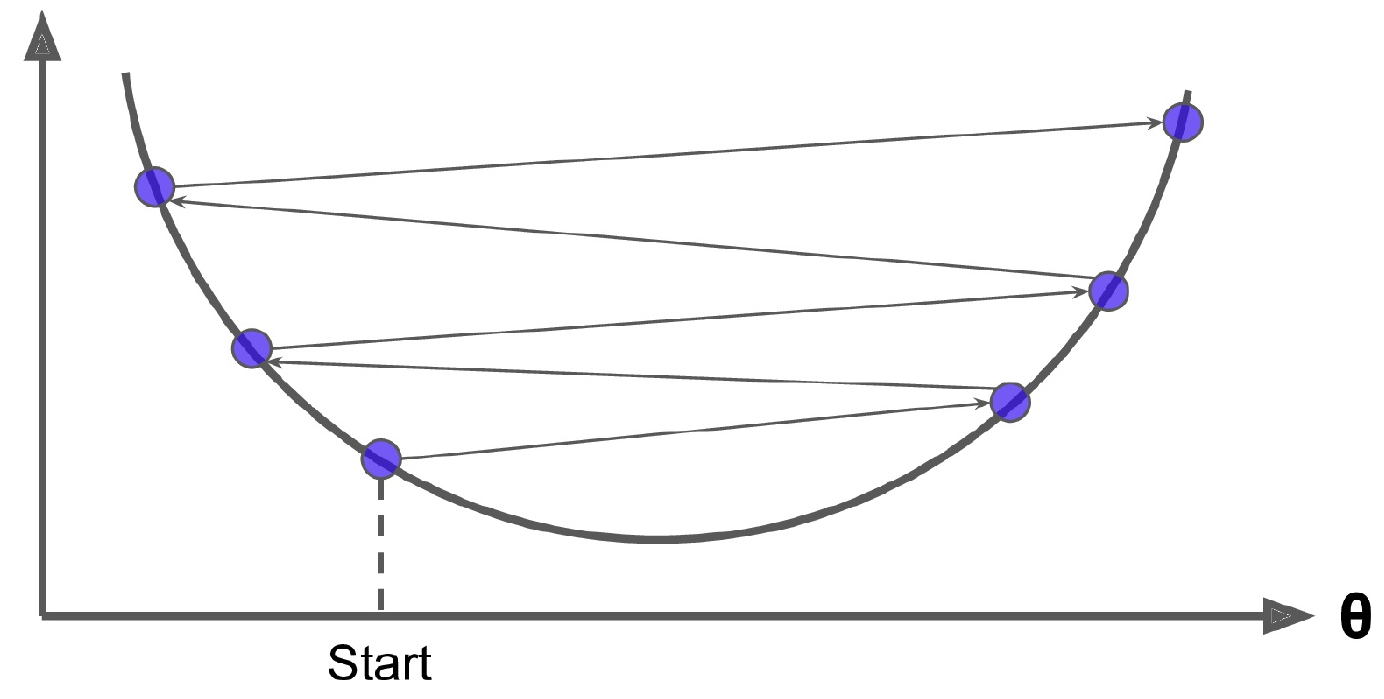
\includegraphics[width=7cm, keepaspectratio]{images/ql_15.png}
\end{center}
\end{column}
\end{columns}
\end{frame}

\begin{frame}{Egyéb problémák}
\begin{columns}
\begin{column}{.5\textwidth}
A gradiens ereszkedés nem garantálja, hogy elér egy globális minimumot, hiszen a gradiens operátora csak lokális változásokat vesz figyelembe. Ebből adódóan az \textbf{algoritmus beragadhat egy lokális minimumon}.\par\medskip
Vannak esetek, amikor a gradiens nem meghatározható (szaturál), például amikor \textbf{elér egy fennsíkot a függvényen}. Ebben az esetben a futás vagy nagyon lassú lesz, vagy nem halad semerre. 
\end{column}
\begin{column}{.5\textwidth}
\begin{center}
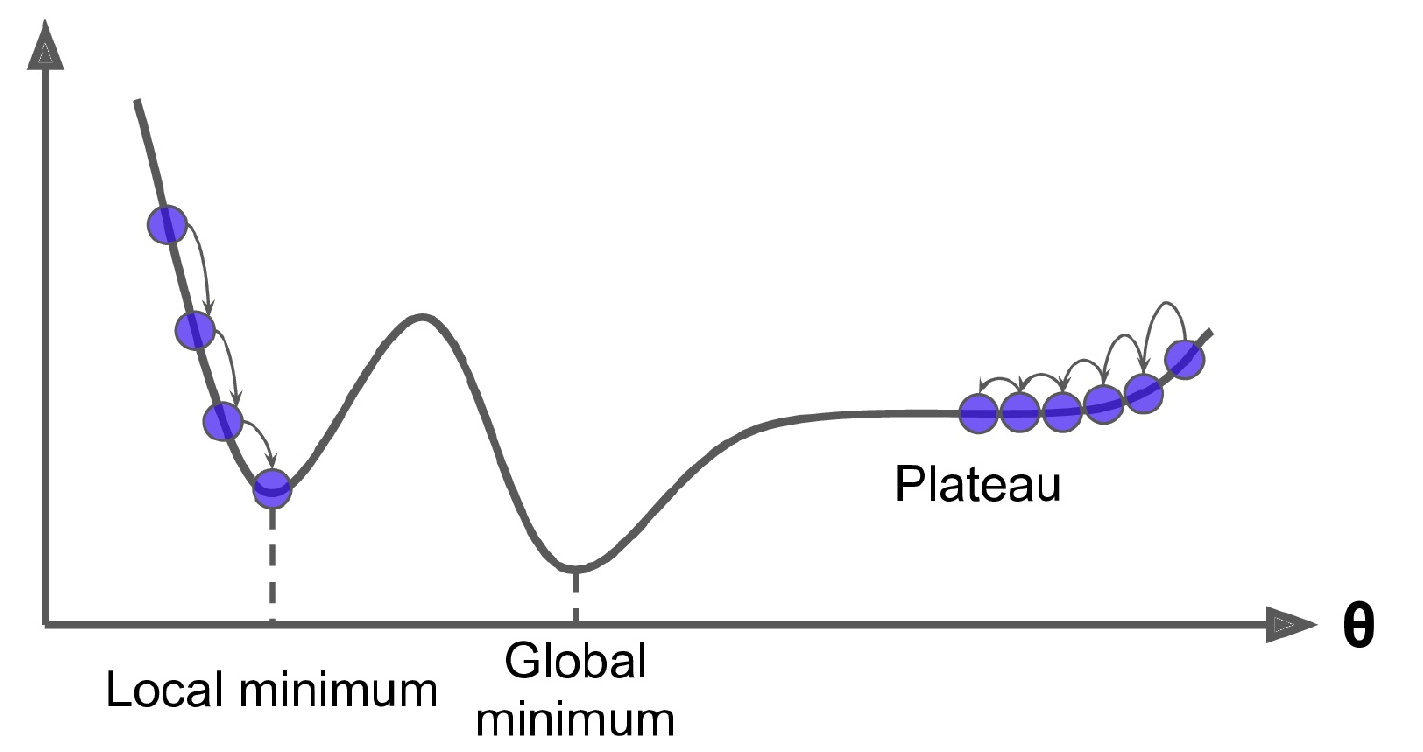
\includegraphics[width=7cm, keepaspectratio]{images/ql_16.png}
\end{center}
\end{column}
\end{columns}
\end{frame}

\section{Neurális hálózatok}

\begin{frame}
\tableofcontents[currentsection]
\end{frame}

\begin{frame}{A neuron}
\begin{columns}
\begin{column}{.4\textwidth}
A neurális hálózatot \textbf{neuronok összessége} alkotja. Az egyes neuronok egyszerű elemi műveleteket végeznek. A neuronnak több inputja (kapcsolata) van, és mindegyikhez egy súly tartozik.\par\smallskip
A neuron kiszámítja az inputjainak a súlyozott összegét ($z=x_1w_1 + x_2w_2 + ... + x_nw_n$), majd ezt az értéket behelyettesíti egy aktivációs függvénybe ($h=\varphi(z)$). 
\end{column}
\begin{column}{.6\textwidth}
\begin{center}
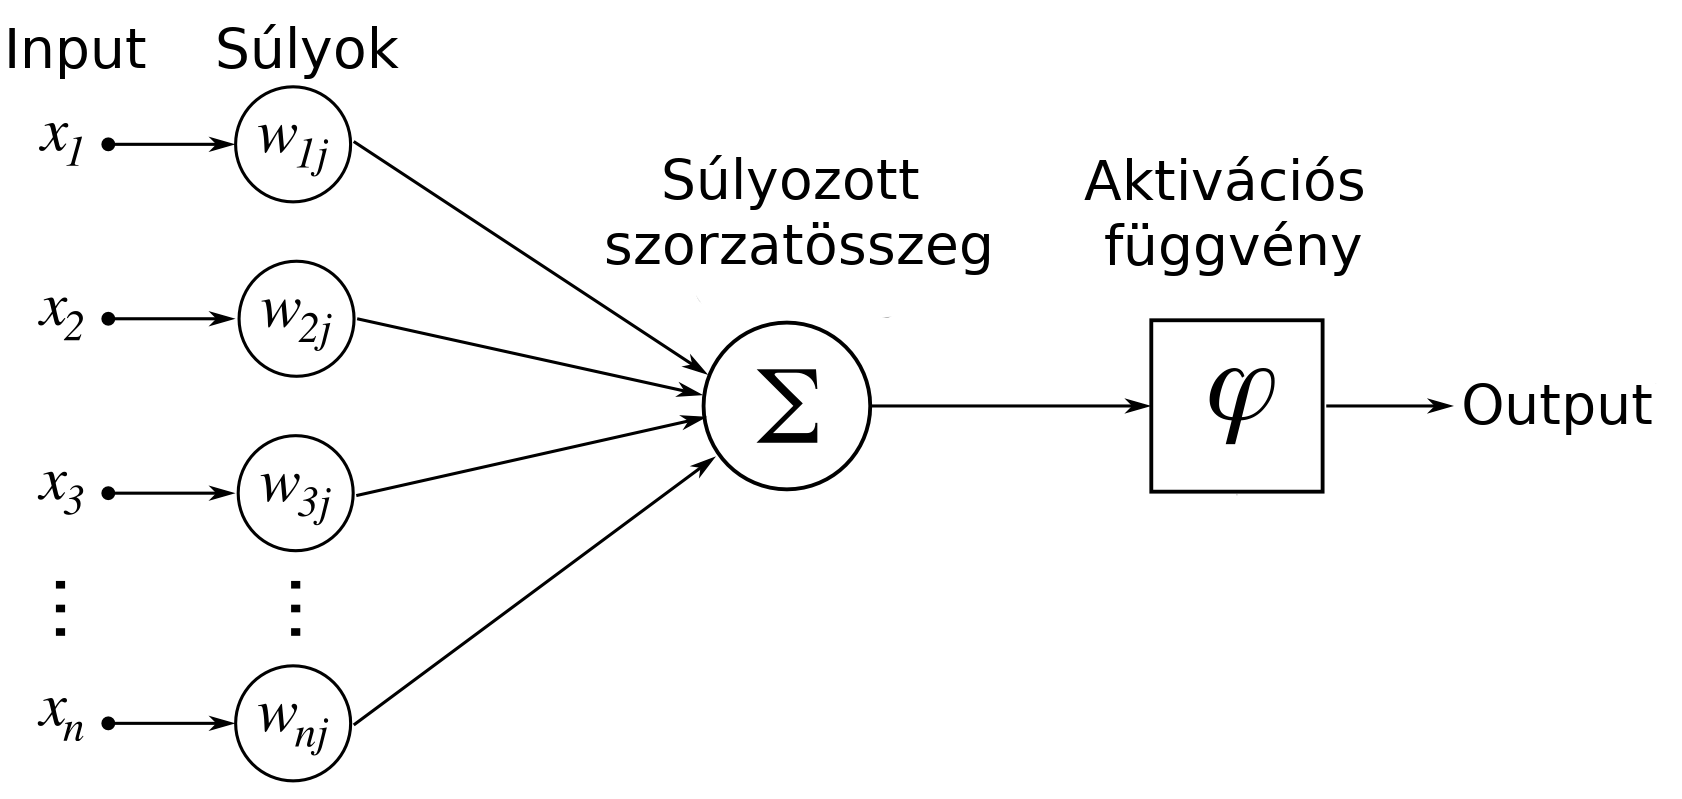
\includegraphics[width=9cm, keepaspectratio]{images/ql_21.png}
\end{center}
\end{column}
\end{columns}
\end{frame}

\begin{frame}{Többrétegű hálózatok}
\begin{columns}
\begin{column}{.5\textwidth}
Ebben az esetben a neuronok rétegekben foglalnak helyet. A kapcsolataik az előző réteg kimeneteivel állnak összeköttetésben. A legelső réteg neuronjai a bemeneti adattal állnak összeköttetésben. Minden bemeneti jellemzőhöz egy neuron tartozik.\par\smallskip
\begin{block}{Teljesen becsatolt neuronréteg kimenete}
\[
h_{W,b}(X)=\varphi(XW+b)
\]
\vspace{-0.5cm}
\begin{itemize}
	\item $X$: Input jellemzők mátrixa
	\item $W$: Kapcsolati súlyok mátrixa
	\item $b$: Torzítások vektora
	\item $\varphi$: Aktivációs függvény
\end{itemize}
\end{block}
\end{column}
\begin{column}{.5\textwidth}
\begin{center}
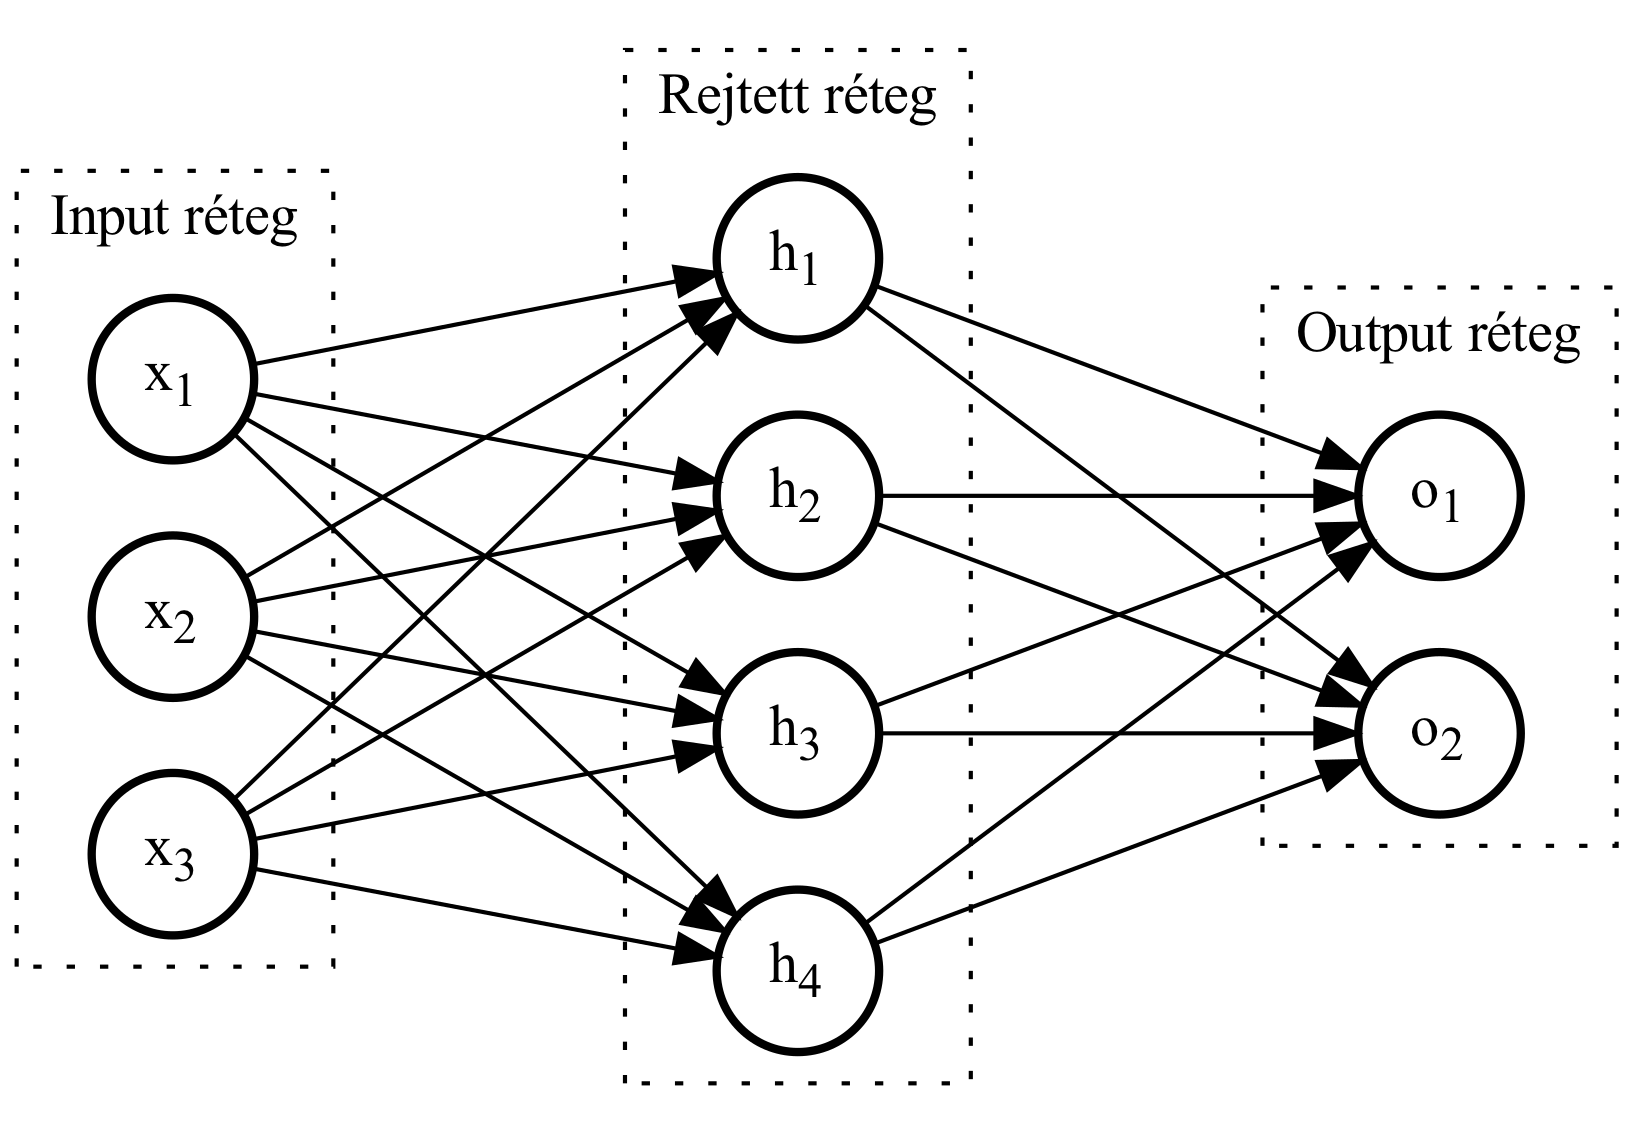
\includegraphics[width=7cm, keepaspectratio]{../../7_dl/doc/graphs/dl_0.png}
\end{center}
\end{column}
\end{columns}
\end{frame}

\section{Mély $Q$-tanulás}

\begin{frame}
\tableofcontents[currentsection]
\end{frame}

\begin{frame}{A $Q$-hálózat (DQN)}
\begin{columns}
\begin{column}{.6\textwidth}
A $Q$-hálózat egy természetes kiterjesztése a hagyományos $Q$-tanulásnak. A naív $Q$-hálózat inputja a \textbf{környezetet leíró változók} vektora vagy mátrixa, és az outputja pedig az ügynök számára elérhető \textbf{cselekvések $Q(s,a)$ értéke} minden $a_1,a_2,..,a_n$ cselekvéshez tartozóan. \par\smallskip
A cselekvés választáshoz az ügynök kiválasztja a legnagyobb becsült $Q$ értéket, és az ahhoz tartozó cselekvést fogja végrehajtani.\par\smallskip
Miután először bemutatták 2013-ban, hamar kiderült hogy a naív $Q$-hálózat nem elég stabil, gyakran eredményez torz politikát a túltanulás miatt. 
\end{column}
\begin{column}{.4\textwidth}
\begin{center}
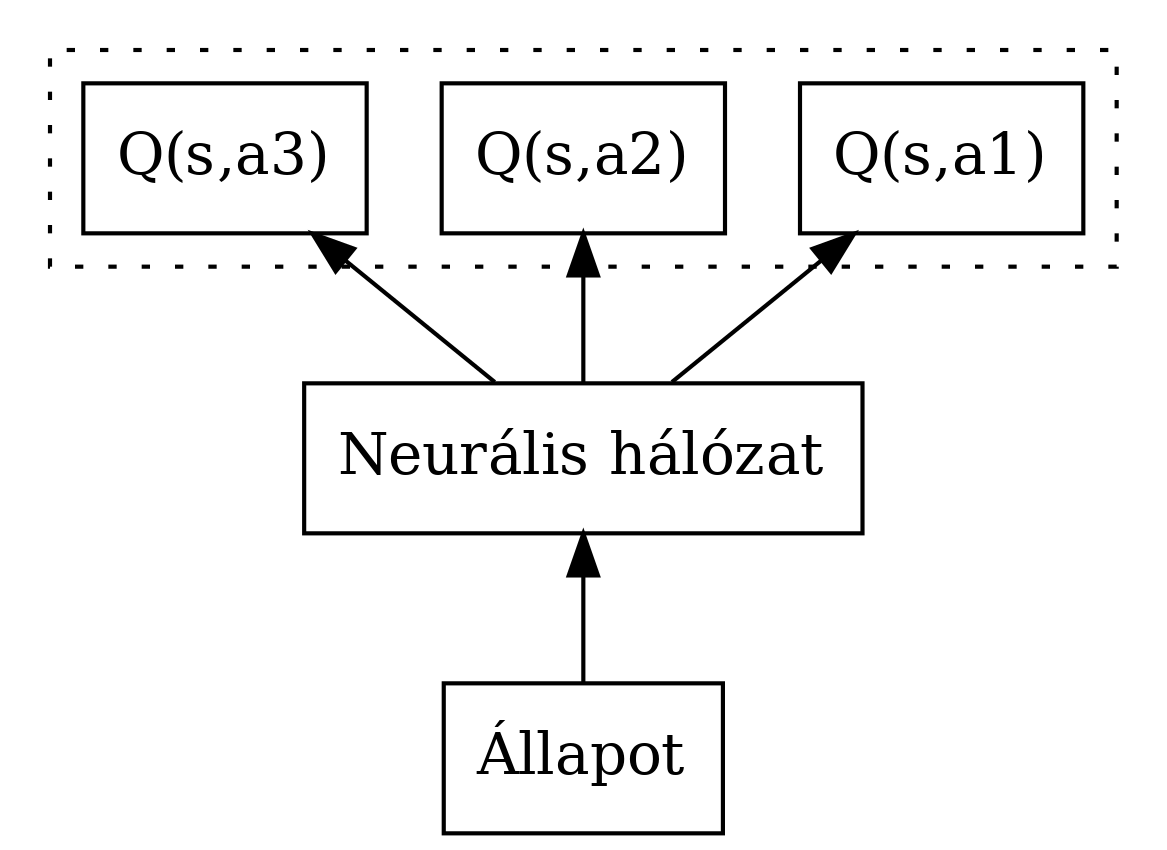
\includegraphics[width=6cm, keepaspectratio]{graphs/ql_3.png}
\end{center}
\end{column}
\end{columns}
\end{frame}

\begin{frame}{Tapasztalat visszajátszás}
\begin{columns}
\begin{column}{.65\textwidth}
A tapasztalat visszajátszás az egyik változtatás, ami a $Q$-hálózat problémáján hivatott segíteni.\par\smallskip
A tapasztalat memória ($D_{replay}$) \textbf{$[s,a,r,s']$ négyeseket tartalmaz}. Minden alkalommal amikor az ügynök cselekszik, az általa tapasztalt $s_t, a_t, r_t, s_{t+1}$ elmentődik a tapasztalat memóriába.\par\smallskip
Amikor tanulásra kerül a sor, az ügynök \textbf{véletlen és rendezetlen mintát} (miniköteget) kap a tapasztalat memóriából, melynek számossága megegyezik a kötegmérettel. Eszerint fogja kiszámolni a költségfüggvényt majd frissíteni a neurális hálózat paramétereit.
\end{column}
\begin{column}{.35\textwidth}
\begin{center}
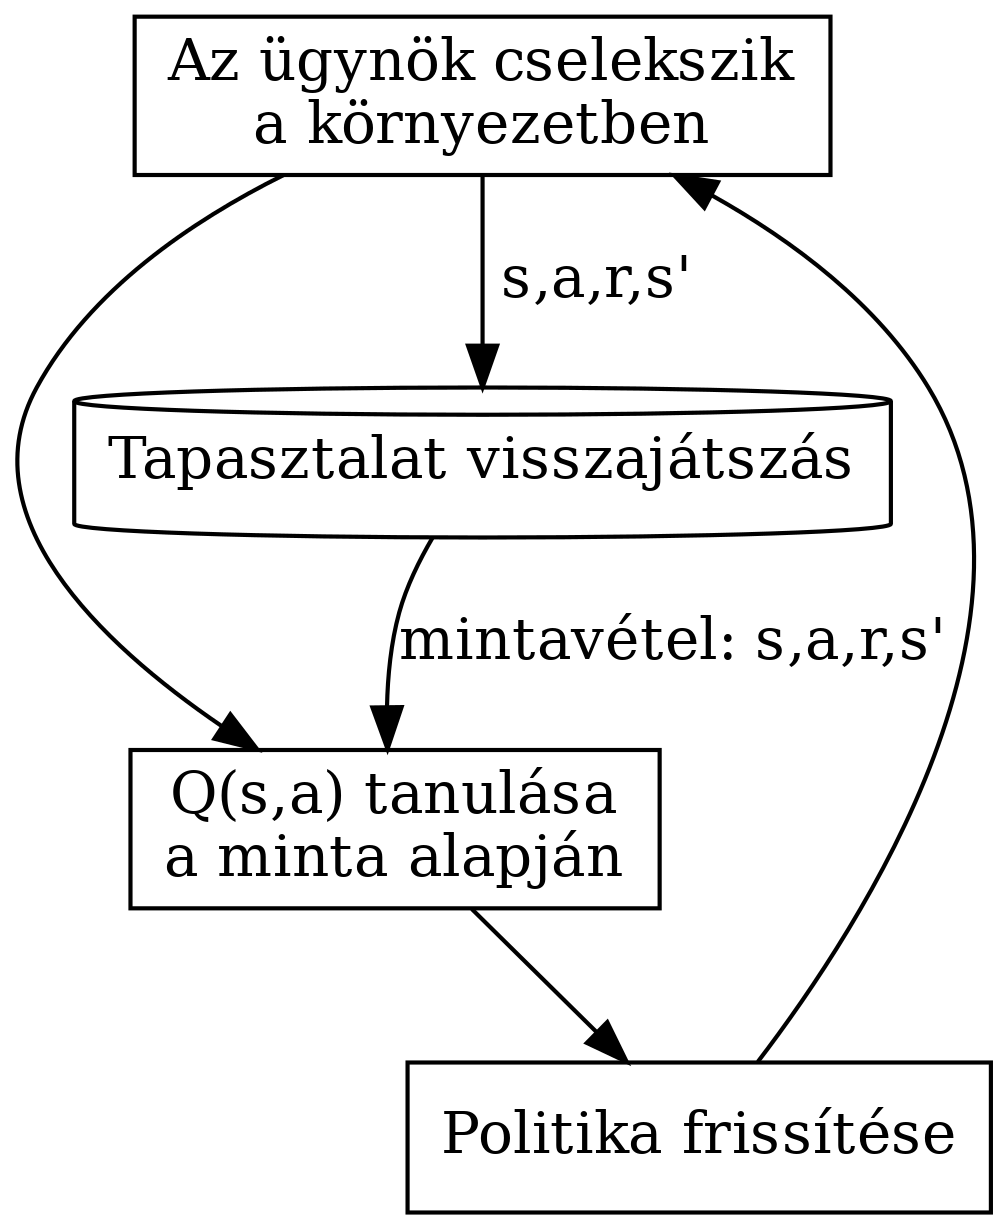
\includegraphics[height=7cm, keepaspectratio]{graphs/ql_4.png}
\end{center}
\end{column}
\end{columns}
\end{frame}

\begin{frame}{Költségfüggvény és frissítési szabály}
\begin{block}{A DQN költségfüggvénye}
\[
J(\theta) = E_{s,a,r,s' \sim D} \left[ \left( r + \gamma \underset{a'}{max} Q_\theta(s',a') - Q_\theta(s,a) \right)^2 \right]
\]
A költségfüggvény a \textbf{négyzetes Bellman hiba várható értéke}. Ahol $s,a,r,s'$ a $D$ \textbf{tapasztalat visszajátszásból vett minta}. $Q_\theta$ megkeresi az $s'$ következő állapothoz tartozó legnagyobb cselekvés értéket (\textbf{célérték}), és lekérdezi $s$ aktuális állapothoz és $a$ aktuális cselekvéshez tartozó értéket. 
\end{block}
\begin{block}{A DQN paraméter frissítése}
\[
\theta' \leftarrow \theta + \alpha \; J(\theta) \; \nabla_\theta Q_\theta(s,a)
\]
Ahol $\theta$ a paramétervektor, $\alpha$ a tanulási sebesség, $J(\theta)$ a költségfüggvény $\theta$ szerint és $\nabla_\theta$ a költségfüggvény gradiense $\theta$ szerint.
\end{block}
\end{frame}

\end{document}












